\documentclass{report}

\usepackage[italian]{babel}
\usepackage[a4paper,top=2cm,bottom=2cm,left=2cm,right=2cm,marginparwidth=1.75cm]{geometry}

\usepackage{amsmath}
\usepackage{graphicx}
\usepackage[colorlinks=true, allcolors=blue]{hyperref}
\usepackage{svg}
\usepackage{subcaption}
\usepackage{wallpaper}
\usepackage{emptypage}
\usepackage[none]{hyphenat}
\usepackage{listings}
\usepackage{xcolor}
\usepackage[chapter]{minted}
\usepackage{verbments}
\usepackage{dirtytalk}
\usepackage{xstring}
\usepackage{fontspec}
\newfontfamily{\noto}{Noto Serif}
\sloppy

\usepackage[backend=bibtex, maxbibnames=10,
minalphanames=3]{biblatex}
\bibliography{Biblio/biblio} 


\title{Editing di ontologie tramite il linguaggio di programmazione funzionale \cduce}
\author{Davide Camino}
\newcommand{\supervisor}{Professoressa Viviana Bono}
\newcommand{\addocaml}[3] {
	\begin{listing}[H]
		\caption{#1}
		\label{#2}
	\end{listing}
	\vspace{-.5cm}
	\inputminted[tabsize=2, linenos, breaklines, bgcolor=bg, escapeinside=~~]{OCaml}{"#3"}
}
\newcommand{\addxml}[3] {
	\begin{listing}[H]%\newcommand{\cduce}{{\fira ℂ}Duce }
		\caption{#1}
		\label{#2}
	\end{listing}
	\vspace{-.5cm}
	\inputminted[tabsize=2, linenos, breaklines, bgcolor=bg]{XML}{"#3"}
}
\newcommand{\cduce}{{\noto ℂ}Duce }
%\newcommand{\cduce}{CDuce }
\renewcommand{\listoflistingscaption}{Elenco listati}
\renewcommand{\listingscaption}{Listato}

\definecolor{bg}{rgb}{0.95,0.95,0.95}


\begin{document}
	\begin{titlepage}
	
	% solo il frontespizio deve essere simmetrico rispetto ai margini interno ed esterno
	\newgeometry{hmargin=2.5cm,vmargin=2.5cm}
	\ThisLLCornerWallPaper{1}{Picture/logoOld2.pdf}
	\begin{figure}
		\centering
			
\includegraphics[width=\textwidth]{Picture/loghi.pdf}
	\end{figure}
	
	\vspace*{\stretch{0.5}}
	
	\begin{center}
		\makeatletter % serve per poter usare \@...
		
		% NOTA: il Times New Roman non supporta il maiuscoletto.
		\textsc{UNIVERSITÀ DI TORINO DIPARTIMENTO DI INFORMATICA}\\
		\vspace*{\stretch{0.1}}
		\textsc{CORSO DI LAUREA TRIENNALE IN INFORMATICA}
		
		\vspace*{\stretch{0.5}}
		\LARGE
		\textbf{\@title}
		
		\vspace*{\stretch{1}}
		\normalsize
		\begin{tabular*}{\textwidth}{l @{\extracolsep{\fill}} r}
			\textbf{Relatore} & \textbf{Laureando} \\
			\supervisor       & \@author           \\
			                  & Matricola: 897753
			\\
		\end{tabular*}
		
		\vspace*{\stretch{2}}
		\textsc{ANNO ACCADEMICO 2022-2023} \\
		\vspace*{\stretch{0.1}}
		Data di laurea 14 Novembre 2023
		
		\makeatother % serve dopo \makeatletter
	\end{center}
	\restoregeometry
\end{titlepage}
	\begin{titlepage}
	\begin{tabular*}{\textwidth}{l @{\extracolsep{\fill}} r}
		 &  \\
		\\
	\end{tabular*}
\end{titlepage}
	\pagenumbering{roman}
	\newgeometry{hmargin=4.5cm,vmargin=2.5cm}
\vspace*{5cm}
\begin{flushright}
    \textit{A tutti quelli che mi vogliono bene.}
\end{flushright}
\vspace{2cm}
\begin{flushright}
	\textit{L'informatica riguarda i computer\\
		non più di quanto l'astronomia riguardi i telescopi.\\
		E. W. Dijkstra}\\
\end{flushright}
\vspace{11cm}
\textit{Dichiaro di essere responsabile del contenuto dell’elaborato che presento al fine del
	conseguimento del titolo, di non avere plagiato in tutto o in parte il lavoro prodotto
	da altri e di aver citato le fonti originali in modo congruente alle normative vigenti in
	materia di plagio e di diritto d’autore. Sono inoltre consapevole che nel caso la mia
	dichiarazione risultasse mendace, potrei incorrere nelle sanzioni previste dalla legge e
	la mia ammissione alla prova finale potrebbe essere negata.}
\vspace{\stretch{4}}
\restoregeometry


	\cleardoublepage
		\begin{tabular*}{\textwidth}{l @{\extracolsep{\fill}} r}
		 &  \\
	\end{tabular*}
	\newpage
	\newgeometry{hmargin=3.5cm,vmargin=4cm}
\chapter*{ABSTRACT}
\addcontentsline{toc}{chapter}{ABSTRACT}
\vspace{1cm}
Questo lavoro illustra lo sviluppo di strumenti per l’editing di ontologie tramite il linguaggio di programmazione funzionale \cduce, in particolare la realizzazione di programmi per il refactoring, il merge e la traduzione da tesauri a ontologie. Lo scopo dello studio è quello di valutare se, e in che condizioni, lo sviluppo di strumenti più o meno ad hoc per l’editing di ontologie sia vantaggioso rispetto all’uso di strumenti grafici tradizionali come Protégé. Nella valutazione si tengono in considerazione principalmente la difficoltà tecnica e il tempo di sviluppo degli strumenti creati con \cduce e il tempo necessario e la ripetitività per fare le stesse modifiche con strumenti grafici.
	\cleardoublepage
		\begin{tabular*}{\textwidth}{l @{\extracolsep{\fill}} r}
		 &  \\
	\end{tabular*}
	\newpage
	\tableofcontents
	\cleardoublepage
	\pagenumbering{arabic}
	\chapter{Concetti di base}

\section*{Introduzione}
Qui illustriamo alcuni dei concetti di base che serviranno per comprendere il resto della discussione, daremo una definizione di ontologia e tesauro, descriveremo brevemente gli strumenti utilizzati e i linguaggi con cui si descrivono le basi di conoscenza che tratteremo.


\section{Basi di conoscenza}
Una base di conoscenza (Knowledge Base KB) è un insieme di affermazioni, ognuna delle quali espressa attraverso un linguaggio di rappresentazione della conoscenza. Le affermazioni esprimono concetti riguardanti il dominio di interesse.

Perché una base di conoscenza possa essere utile deve essere possibile aggiungere conoscenza (fare affermazioni) e interrogare la KB; queste operazioni possono coinvolgere meccanismi di inferenza che permettano di ricavare nuove affermazioni da quelle già note. L'inferenza sfrutta una logica formale per ricavare nuove informazioni partendo da quelle che sono già presenti nella KB.\cite{russell2010artificial}
\subsection{Ontologie}
\subsubsection{Definizione}
In accordo con una definizione ampiamente accettata \cite{hitzler2021review} un'ontologia ha lo scopo di rappresentare un vocabolario per definire i concetti di un particoare dominio di interesse condiviso, ed è costituita da definizioni di classi, relazioni, funzioni e altri oggetti utili a rappresentare la conoscenza\cite{gruber1993translation}. 

La definizione è ancora un po' vaga, più precisamente un'ontologia è una base di conoscenza che permette di descrivere concetti e relazioni tra di essi specificando questi oggetti tramite un linguaggio di rappresentazione della conoscenza basato su una logica formale.
\subsubsection{Scopo delle ontologie}
Nel contesto del web semantico\footnote{Un'estensione del World Wide Web in cui le informazioni siano comprensibili ad un automa\cite{berners2001new}} le ontologie sono il mezzo principale per condividere, integrare e scoprire dati\cite{hitzler2021review}.
\subsubsection{Manipolare ontologie}
 Dato lo scopo delle ontologie risulta essere un argomento centrale la possibilità di riutilizzare, modificare e ampliare ontologie esistenti. Spesso le basi di conoscenza sono sì strutturate, ma sono eterogenee e non permettono interoperabilità. Scopo di questo lavoro è quello di presentare degli strumenti per manipolare basi di conoscenza (ci concentriamo si tesauri e ontologie) operando in modo tale da rendere compatibili informazioni tratte da fonti differenti. 
 
 Il testo \cite{suarez2015neon} presenta una trattazione teorica approfondita sulle metodologie per sviluppare un'ontologia, in particolare il framework NeOn prevede vari scenari tipici in cui ci si può trovare quando si voglia costruire un ontologia, si fa particolare attenzione ai casi nei quali siano già presenti informazioni, ma queste vanno riorganizzate.
\subsubsection{Esempio}
Consideriamo una semplice ontologia che rappresenta persone con legami di parentela genitore-figlio; le persone hanno uno o più nomi salvat nel tag \verb|comment|. Modelliamo questa ontologia con una classe \verb|Persone| e una sottoclasse \verb|Genitori| (i cui individui sono \verb|Persone| che realizzano la relazione \verb|genitoreDi|). Creiamo la relazione \verb|genitoreDi|. Infine popoliamo l'ontologia con alcuni individui. Il risultato ottenuto con Protégé è un documento XML di questo tipo:
\addxml{persone.rdf}{lst:persone.rdf}{Code/persone.rdf}
Per quanto non sia impossibile leggere la struttura e i dati dal listato precedente un modo naturale per rappresentare le ontologie è sotto forma di grafi. Qui vediamo il grafo\footnote{tutti i grafi presenti un questo elaborato sono stati ottenuti grazie a http://vowl.visualdataweb.org/webvowl.html} che mostra la struttura dell'ontologia e possiamo apprezzare quanto sia semplice la sua struttura rispetto a quello che avremmo potuto immaginare dal listato \ref{lst:persone.rdf}. Nel grafo non sono rappresentati gli individui, possiamo comunque leggere quanti ve ne sono per ogni classe (in questo caso un individuo di tipo \verb|Persone| e uno di tipo \verb|Genitori|)
\begin{figure}[H]
	\centering
	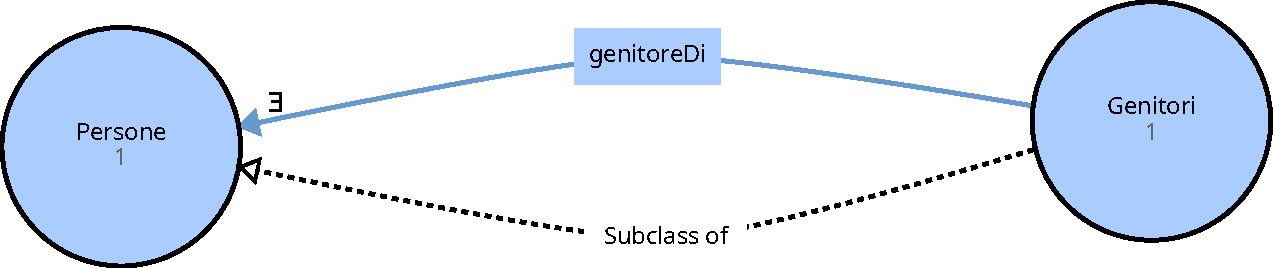
\includegraphics[width=0.5\textwidth]{Picture/persone.rdf.pdf}
	\caption{Grafo dell'ontologia persone}
\end{figure}


\subsection{Tesauri}
\subsubsection{Definizione}
Nella loro accezione più generale possibile i tesauri sono risorse nelle quali termini affini sono raggruppati assieme\cite{kilgarriff2000s}. In particolare un tesauro fornisce un vocabolario preciso e controllato rispetto ad un particolare dominio di interesse.\cite{srinivasan1992thesaurus} Queste strutture possono aiutare il ricercatore a riformulare le strategie di ricerca fornendo una serie di sinonimi, contrari, definizioni e traduzioni in altre lingue del termine cercato.

Esistono diversi tipi di tesauro in base alle modalità di costruzione e fruizione \cite{kilgarriff2000s}, nel nostro caso il tesauro sarà costituito da un vocabolario tassonomico in cui le relazioni tra oggetti sono di tipo BT (broader term), cioè ogni concetto può avere un riferimento ad un concetto più generale, formando in questo modo una struttura ad albero. 
\subsubsection{Espressività}
Come si può immaginare il potere espressivo di un tesauro è inferiore a quello di un'ontologia che non pone alcun limite alle relazioni definibili tra individui. In un tesauro inoltre ogni concetto ha al più un genitore, mentre in un ontologia possiamo creare una classe che erediti le caratteristiche da più classi distinte.
\section{Strumenti di editing}

\subsection{Protégé}
Protégé\footnote{https://protege.stanford.edu/} è uno strumento per la modellazione della conoscenza molto conosciuto; è un progetto open-source sviluppato all'università di Stanford e permette la manipolazione interattiva di ontologie e KB attraverso un'interfaccia grafica e delle API java.

Le funzionalità di Protégé possono essere aumentate grazie a dei componenti plug-in il cui numero è in continua crescita. Questi plug-in offrono nuovi metodi per la gestione delle ontologie, supporto per dati multimediali, engines per il ragionamento automatico e per l'interrogazione delle basi di conoscenza\cite{sivakumar2011ontology}.
\subsubsection{Descrizione del software}
Protégé presenta un'interfaccia con numerose schede, ogni scheda permette all'utente di accedere ad una differente funzionalità del software. Le schede base consentono di aggiungere nuova conoscenza e di effettuare ricerche nella KB.

Uno degli obbiettivi fondamentali di Protégé è quello di rendere l'inserimento e la ricerca in una base di conoscenza il più semplice possibile: mentre il sistema genera uno strumento per l'acquisizione della conoscenza l'utente aggiunge informazioni riempiendo form intuitivi, selezionando elementi da delle liste e disegnando diagrammi.

Protégé permette di salvare le ontologie in numerosi formati, tra cui UML, XML, RDF e OWL.
\begin{figure}[h]
	\centering
	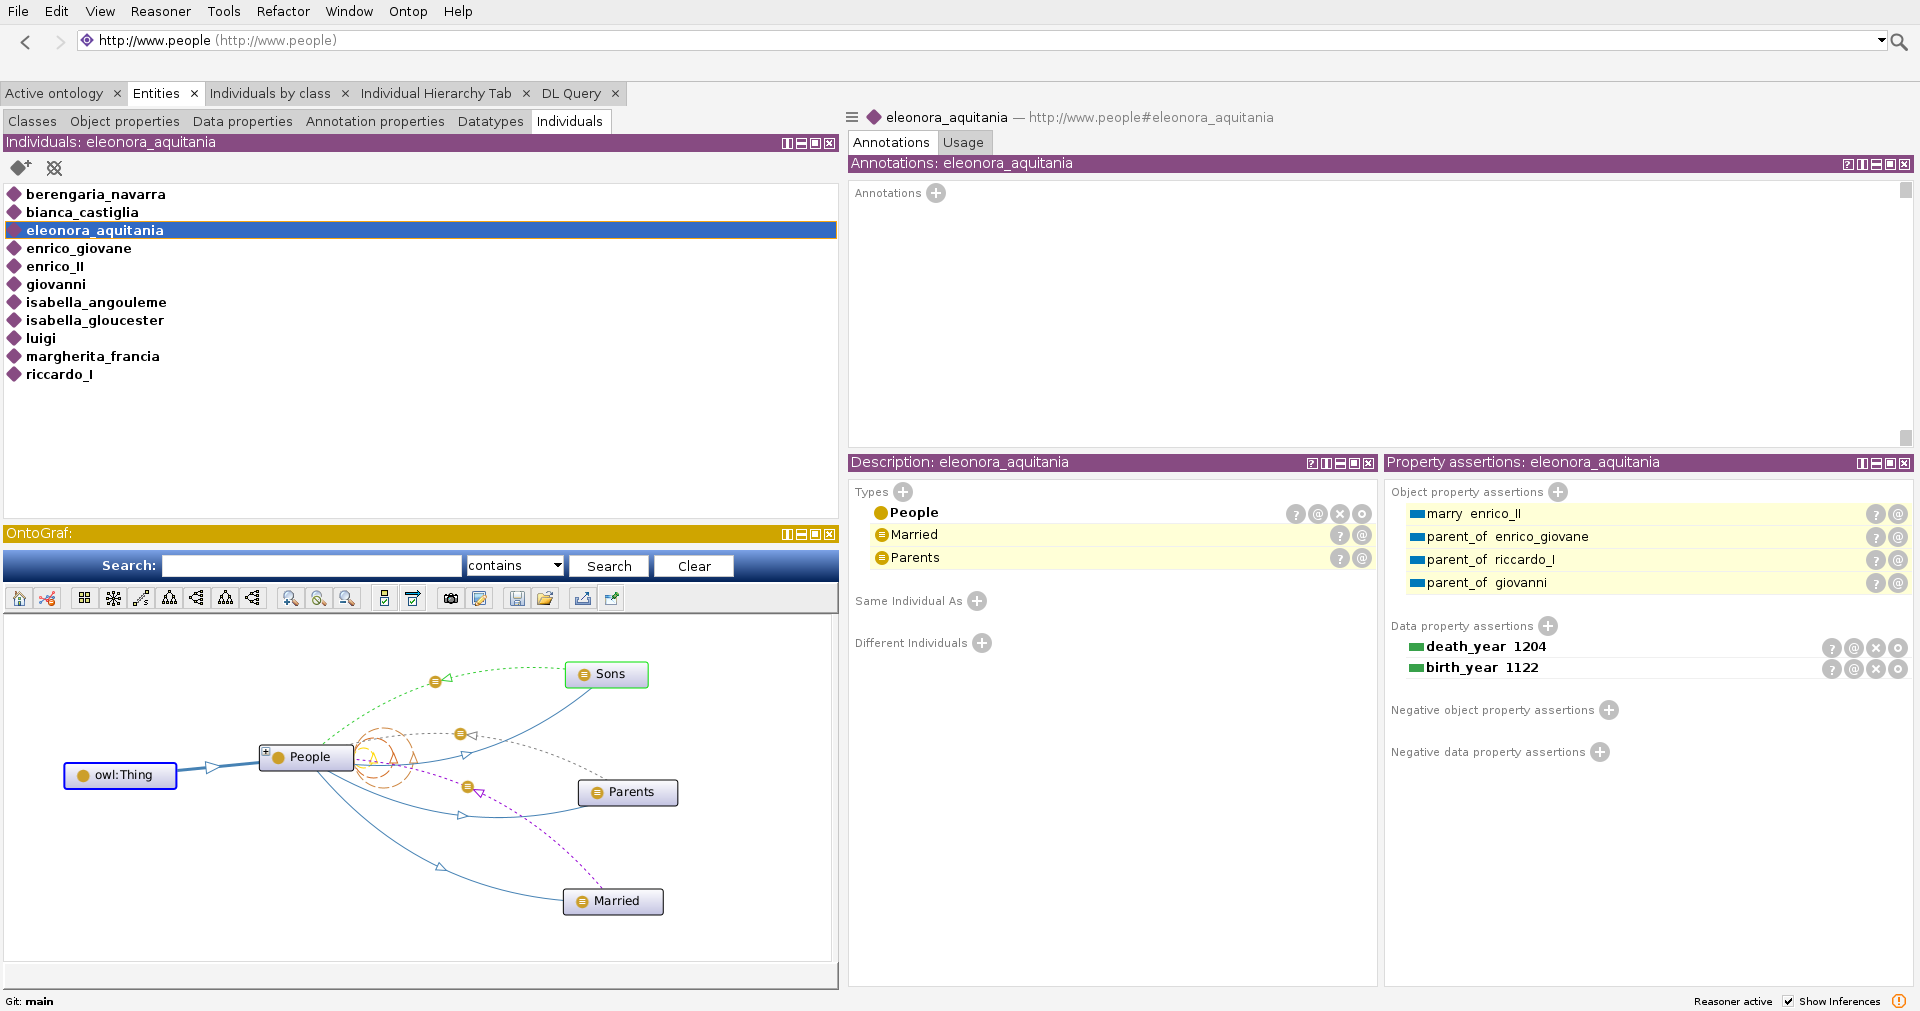
\includegraphics[width=\textwidth]{Picture/interface_protege.png}
	\caption{Interfaccia di Protégé}
\end{figure}
\subsection{\cduce}
\cduce è un linguaggio di programmazione funzionale, staticamente tipato e orientato allo sviluppo di applicazioni che lavorano su documenti XML\cite{cduceLanguage}, nasce con líntento di migliorare XDuce: un altro linguaggio di programmazione per il processing di file XML\cite{hosoya2003xduce}. 

XDuce permette di manipolare unicamente documenti XML, questa sua specificità mostra come la presenza di feature mirate possano aiutare e semplificare lo sviluppo di applicazioni XML sacrificando, però, la possibiltà di scrivere applicazioni complesse in cui non si facciano solo semplici trasformazioni di elementi XML.

\cduce si pone l'obbiettivo di integrare specifiche funzioni orientate alla manipolazione XML all'interno di un linguaggio potenzialmente general-porpouse. Per fare questo \cduce usa un algebra general-porpouse, con costruttori di tipo standard mantendendo l'espressività e la potenza delle espressioni regolari di XDuce attraverso l'uso di tipi ricorsivi e combinatori logici (unione, intersezione, differenza).

In \cduce è possibile creare complesse strutture dati, modellare il tipo di documenti XML, e interfacciarsi in modo relativamente semplice con altri linguaggi di programmazione\cite{cduceLanguage}.
\subsection{Feature}\label{fature_cduce}
Vediamo brevemente le principali feature di \cduce, non entreremo nel dettaglio essendo presente una guida dettagliata sul sito del progetto\footnote{https://www.cduce.org/}
\subsubsection{Verifica statica dei tipi}
Il sistema di tipi è un componente centrale di \cduce; dal punto di vista pratico un tipo è un insieme di valori identificati da un espressione sintattica, questa descrizione di un tipo permette di definire in modo naturale (come insiemi matematici) relazioni di sottotipo, connettivi logici nell'algebra dei tipi ed equivalenza di tipi.

I tipi ricoprono un ruolo importante anche nella parte statica del linguaggio: la correttezza di ogni trasformazione definita in \cduce è garantita staticamente. Inoltre in \cduce il pattern matching viene effettuato attraverso un esatta inferenza di tipo, nel senso che viene assegnata ad ogni variabile legata esattamente il set di tutti i valori che questa può assumere.

In questo modo è possibile costruire in sistema di tipi statico e molto preciso, che permette una migliore descrizione del comportamento dinamico del programma sviluppato
\subsubsection{Pattern matching}
\label{CDucePattern}
È un'operazione fondamentale in \cduce ed ha la forma:
\begin{minted}[tabsize=2, breaklines, bgcolor=bg]{OCaml}
match e with
	| p1 -> e1
	...
	| pn -> en
\end{minted}
Si cerca di fare il match tra la valutazione di un'espressione \verb|e| e vari pattern \verb|pi|. Il primo pattern che fa il match con \verb|e| attiva la corrispondente espressione sulla destra che può usare le variabili legate dal pattern.

Il controllo statico dei tipi si assicura che il pattern matching sia esaustivo, il tipo valutato per \verb|e| deve essere sottotipo dell'unione dei tipi accettati dai pattern definiti sotto.
\subsubsection{Funzioni}
La forma generale di una funzione è
\begin{minted}[tabsize=2, breaklines, bgcolor=bg]{OCaml}
fun myfunc (t1 -> s1; ...; tn -> sn)
	| p1 -> e1
	...
	| pm -> em
\end{minted}
In cui la prima riga è l'interfaccia della funzione, il rimanente è detto corpo:
\begin{itemize}
	\item interfaccia: rappresenta il modo in cui la funzione si comporta: quando riceve un elemento di tipo \verb|ti| la funzione restituirà un elemento di tipo \verb|si|, per ogni clausola \verb|ti -> si| il sistema verifica che la funzione trasformi correttamente gli elementi;
	\item corpo della funzione: le funzioni operano per pattern matching degli argomenti: viene eseguita la prima trasformazione tale che l'argomento ricevuto come parametro faccia il match col pattern \verb|pi|. 
\end{itemize}
In \cduce è possibile definire anche applicazioni parziali(curried functions\footnote{https://en.wikipedia.org/wiki/Currying}) e funzioni di ordine superiore\footnote{https://en.wikipedia.org/wiki/Higher-order\_function}
\section{Metalinguaggi}
Un metalinguaggio è in generale un linguaggio , o sistema di segni, naturale o artificiale, adottato per la descrizione della struttura formale di dati linguaggi\footnote{https://www.treccani.it/vocabolario/metalinguaggio}. In questo elaborato parliamo di linguaggi su tre differenti livelli:
\begin{itemize}
	\item linguaggi di programmazione: sono i linguaggi con i quali sviluppiamo strumenti più o meno automatici per la manipolazione di basi di conoscenza;
	\item ontologie e tesauri: esprimono della conoscenza in modo formale, rispettano certe logiche per poter essere usate e restituiscono all'interrogatore una risposta che quest'ultimo sia in grado di comprendere
	\item linguaggi per descrivere le basi di conoscenza: abbiamo bisogno di un linguaggio per descrivere la struttura di una KB, per definire quali relazioni possono esserci e in generale per parlare le KB stessa; chiameremo questi ultimi metalinguaggi\footnote{questi linguaggi non ci permettono di descrivere il dominio di interesse di per sè ma descrivono come descrivere il dominio} per distinguerli dai linguaggi di programmazione e dalla conoscenza che stiamo rappresentando.
\end{itemize}
Presentiamo alcuni metalinguaggi importanti che useremo per descrivere ontologie e tesauri.
\subsection{XML}
XML (Extensible Markup Language) è un formato testuale semplice e molto flessibile, inizialmente ideato per far fronte alla pubblicazione digitale su larga scala e diventato col tempo uno strumento importantissimo per lo scambio di moltissime informazioni sul Web\cite{w3cXml}.

I documenti XML servono per memorizzare elementi detti entità che contengono dati formattati e non. I dati formattati sono costituiti da due componenti: il dato stesso e una parte di markup; quest'ultimo codifica la descrizione logica e la struttura di memorizzazione del documento. XML consente di imporre regole alla struttura logica e di memorizzazione del documento\cite{world2006extensible}.

Per una descrizione dettagliata delle specifiche di XML si rimanda a \cite{world2006extensible}, mentre \cite{li2005testing} illustra nei particolari caratteristiche e funzionalità dello Schema XML. Ci limitiamo qui a definire la struttura di un elemento XML: \verb|<(tag) (attr)>content</(tag)>| e a fornire un esempio di un'entità che potremmo trovare in un documento XML:
\begin{minted}[tabsize=2, breaklines, bgcolor=bg]{XML}
<person gender="F">
	<name>Clara</name>
	<children>
		<person gender="M">
			<name>Bob</name>
			<children/>
		</person>
	</children>
	<email>clara@lri.fr</email>
	<tel>314-1592654</tel>
</person>
\end{minted}
Questa entità descrive una donna di nome Clara, che ha un figlio maschio di nome Bob, attribuiamo a Clara anche un numero di telefono e una e-mail.

Alla luce di questa descrizione si può provare a reinterpretare il listato \ref{lst:persone.rdf} che descrive la relazione di parentela tra Giulio Cesare e Bruto.
\subsection{RDF/RDFS}
\subsubsection{RDF}
RDF (Resource Description Framework) è un framework (architettura logica che supporta una prassi, una metodologia o un progetto\footnote{https://it.wikipedia.org/wiki/Framework}, in questo caso definisce le regole per la descrizione della conoscenza) per il processing di metadati\footnote{esattamente come i metalinguaggi i metadati sono dati che descrivono altri dati}. RDF permette l'interoperabilità tra applicazioni che si scambiano informazioni comprensibili ad un automa.

Lo scopo di RDF è quello di automatizzare il processing di risorse Web; trova quindi applicazione nella ricerca di informazioni permettendo un motore di ricerca migliore, in applicazioni che catalogano la conoscenza, per descrivere una collezione di pagine che rappresentano un unico \say{documento} logico, ecc...\cite{brickley1998resource}

RDF si basa sull'idea di rappresentare oggetti attraverso identificatori Web (URI\footnote{Uniform Resource Identifiers}) e di descrivere le risorse in termini di semplici proprietà e valori. I valori possono essere tipi semplici (numeri caratteri stringhe) oppure altre risorse identificate con URI.

RDF permette quindi di esprimere semplici affermazioni riguardo risorse attraverso grafi i cui nodi rappresentano risorse e i cui archi rappresentano proprietà e valori\cite{manola2004rdf}.
\subsubsection{RDFS}
Uno Schema RDF definisce quali siano le proprietà valide che si possono esprimere in una particoloare descrizione con RDF; permette inoltre di imporre caratteristiche o restrizioni alle proprietà e ai valori che queste possono assumere. Per identificare uno Schema RDF viene usato il meccanismo dei namespace XML\footnote{Una serie di nomi, identificati da un URI usati in un documento XML come tipi di un elemento e nomi di attributi\cite{bray1999namespaces}}.

Interpretare uno Schema RDF significa attribuire un valore semantico ad ogni proprietà presente nella descrizione RDF, questo significa che anche se un'applicazione non è in grado di capire lo schema può comunque ricostruire il grafo di risorse descritto da RDF\cite{miller1998introduction}.
\subsection{OWL}
L'espressività di RDF e RDFS è limitata, potendo descrivere somo predicati binari, una struttura delle classi gerarchica e proprietà anch'esse gerarchiche con un dominio e un codominio.

Sono state individuate dal gruppo di ricerca \say{Web Ontology Working Group} una serie di casi in cui le ontologie devono poter essere descritte con linguaggi più espressivi rispeto a RDF e RDFS\cite{antoniou2009web}.

Presentiamo le funzionalità aggiunte da OWL Full: la versione più espressiva\footnote{e anche più pesante computazionalmente} del linguaggio OWL; per una descrizione più approfondita del linguaggio si rimanda al documento prodotto da W3C a riguardo\footnote{https://www.w3.org/TR/2004/REC-owl-features-20040210}.
\subsubsection{OWL Full}
Presenta la compatibilità massima coi documenti RDF/RDFS, ha la massima espressività, ma non è un sistema decidibile e completo. Descriviamo questo con il solo scopo di fornire l'elenco più completo possibile di funzionalità aggiunte allo scopo di aumentare l'espressività di RDF/RDFS.

OWL Full\footnote{come anche OWL DL} permette di:
\begin{itemize}
	\item definire restrizioni sui domini delle relazioni in base alla classe (si può limitare ad esempio un individuo di classe mucca a mangiare solo piante, senza applicare la stessa restrizione ad altri animali);
	\item esprimere disgiunzione tra classi;
	\item definire classi tramite operazioni insiemistiche tra altre classi;
	\item definire restrizioni sulla cardinalità di una proprietà
	\item definire caratteristiche particolari di una proprietà come transitività, riflessività, proprietà inversa, ecc...
\end{itemize}

In OWL Full è, inoltre, possibile utilizzare ogni primitiva del linguaggio OWL combinandola con le primitive del linguaggio RDF/RDFS in modo da alterarne il significato originario (applicando anche una primitiva all'altra).
\subsection{SKOS}
SKOS (Simple Knowledge Organization System) è un modello basato su RDF che permette di esprimere la struttura base e il contenuto di schemi concettuali come tesauri, tassonomie e altri tipi di vocabolari affini\cite{isaac2009skos}.

In SKOS i concetti possono essere identificati con URI, etichettati con stringhe di caratteri in una o più lingue, descritti con delle annotazioni, associati ad altri concetti o organizzati in strutture gerarchiche informali\cite{miles2009skos}.

Più avanti vedremo che questo linguaggio è stato usato per descrivere il tesauro \say{Eurpeana Fashion Thesaurus}, questo tesauro è facilmente reperibile online ed è ottimo per i nostri esperimenti di editing (ne parleremo in \ref{ch3}).	
	\chapter{Strumenti offerti da \cduce}\label{ch2}
\section{Introduzione}
In questo capitolo analizziamo brevemente gli strumenti principali offerti da \cduce per l'editing di documenti XML. La trattazione vale per un qualsiasi documento XML, ma negli esempi ci concentreremo sulle ontologie analizzando i primi comandi per trattare ontologie dalla struttura semplice. 


\section{Parsing di documenti XML}
Un documento XML non è altro che una struttura ad albero: ogni nodo rappresenta un concetto che può essere meglio definito nei figli del nodo stesso. 

In \cduce possiamo ricostruire tale struttura definendo dei tipi. La forma generale di un elemento XML è \verb|<(tag) (attr)> content| dove \verb|tag|, \verb|attr| e \verb|content| sono espressioni su cui è possibile fare patten matching. Si può quindi creare un tipo generale che faccia match con il tag root del documento XML e che, come \verb|content|, abbia un array eterogeneo che conterrà tutti i figli del tag root. A ogni elemento del vettore sarà associato un tipo che avrà la stessa struttura del tipo generale e che permetterà di descrivere la struttura del documento XML discendendo fino alle foglie.
\subsection{Esempio}
Torniamo all'esempio dell'ontologia di persone definita nel listato \ref{lst:persone.rdf} e descriviamo in \cduce la sua struttura:
\addocaml{persone.cd}{lst:persone.cd}{Code/persone.cd}
Si definiscono (linea 1 a 6) i namespace in modo che \cduce li possa interpretare correttamente nel resto del documento. Si passa poi alla struttura vera e propria del file: tutte le informazioni sono contenute nell'elemento di tipo \verb|Ontology| che è costituito da un tag e da una lista di elementi di tipo \verb|Thing| che a sua volta può rappresentare un elemento di tipo \verb|Ont|, \verb|Property|, \verb|Class| o \verb|Individual|. Ognuno di questi elementi fa il match con un nodo figlio del nodo root del documento XML; a loro volta questi elementi hanno una struttura interna che può essere più o meno dettagliata a seconda di come ci interessa operare sul documento. È interessante notare che, dato che in questo caso le specifiche proprietà della restrizione di un elemento \verb|EqClass| non ci interessano, abbiamo potuto fare il match di queste con un vettore di lunghezza arbitraria (anche nulla) di generici elementi XML. Se avessimo voluto specificare che il tag restrizione contiene esattamente due elementi senza specificare quali, avremmo potuto scrivere \verb|<owl>Restriction> [AnyXml AnyXml]|.

Quando andremo a caricare il documento con il comando alla riga 26, \cduce carica il file ed esegue il controllo di tipo verificando che la struttura del file XML sia effettivamente quella descritta dall'elemento \verb|Ontology|; se il controllo va a buon fine, otterremo l'elemento chiamato \verb|ontology| di tipo \verb|Ontology| contenente tutto il file XML.
\section{Manipolare documenti XML}
Una volta definita la struttura del documento possiamo definire delle funzioni che mappano un elemento in un altro elemento. Gli strumenti fondamentali sono:
\begin{itemize}
	\item pattern matching: descritto nel paragrafo \ref{CDucePattern}
	\item \verb|map|\label{map}: permette di applicare una funzione a tutti gli elementi di una lista e restituisce una nuova lista di elementi trasformati della stessa lunghezza della lista iniziale;
	\item \verb|transform|: permette di applicare una funzione a ogni elemento di una lista, restituendo per ogni elemento una lista di lunghezza arbitraria (anche nulla) e concatenando infine il risultato. Grazie alla funzione \verb|transform| si può ottenere una lista di lunghezza diversa rispetto alla lista di partenza.
\end{itemize}

\subsection{Esempio}
Consideriamo nuovamente l'ontologia padri-figli con struttura definita in \ref{lst:persone.cd} e costruiamo due funzioni, la prima (chiamata \verb|name|) che permetta di estrarre da un individuo tutti i nomi, la seconda (chiamata \verb|names|) che usi la prima per costruire una lista con tutti i nomi contenuti nell'ontologia.
\addocaml{basic functions}{lst:basic_functions.cd}{Code/basic_func.cd}
Nella prima funzione, usando il pattern matching, si lega la variabile \verb|n| alla sequenza di tutti gli elementi di tipo \verb|Name| associati a quell'individuo, poi si usa \verb|map| per estrarre da ogni elemento di questa lista solo la stringa col nome.

Nella seconda funzione si usa \verb|transform| per selezionare dalla lista \verb|x| (lista di elementi tipo \verb|Thing|) i soli elementi \verb|Individual|, a questi si applica la funzione \verb|name| sopra definita. La seconda clausola di \verb|transform|, che serve a scartare tutti gli elementi di cui non si è ancora fatto il match, è implicita e può essere quindi omessa.

La prima funzione ci ha permesso di passare da una lista \verb|n| di elementi \verb|Name| a una lista della stessa lunghezza di stringhe. La seconda ci ha permesso di passare da una lista di elementi \verb|Thing| a una lista di elementi \verb|Individual| di differente lunghezza (questa lista viene poi trasformata in una lista di stringhe usando la funzione \verb|name|).
\section{Query}
Un punto di forza di \cduce sono le Query. Le useremo profusamente nei capitoli \ref{ch3} e \ref{ch4} per creare liste e selezionare elementi in modo rapido e leggibile al posto della  funzione \verb|transform|.
La forma generale di una Query è molto simile alla stessa espressa in SQL:
\begin{minted}[tabsize=2, bgcolor=bg]{OCaml}
select e 
from p1 in e1,
	 p2 in e2,
	 :
	 pn in en
where c
\end{minted}
Dove \verb|e| ed \verb|ei| sono espressioni, \verb|pi| sono pattern e \verb|c| è un'espressione booleana. Il risultato finale è la lista di tutti i valori ottenuti valutando \verb|e| nella sequenza di possibili combinazioni in cui le variabili libere di \verb|e| sono legate facendo il match dei pattern \verb|pi| con le espressioni \verb|ei|, a condizione che \verb|c| sia rispettata.

Le Query possono essere simulate con \verb|transform| che permette di creare, grazie a pattern matching successivi, l'espressione \verb|e| e di selezionarla solo nel caso in cui l'espressione booleana \verb|c| sia rispettata. Si può riscrivere la generica Query usando la \verb|transform| come segue:
\begin{minted}[tabsize=2, bgcolor=bg]{OCaml}
transform e1 with p1 -> 
	transform e2 with p2 -> 
		...
			transform en with pn -> 
				if c then  [e] else []
\end{minted}
La valutazione dei due comandi produce il medesimo risultato.

Anche se \verb|transform| può sembrare più versatile o espressiva delle Query, quando possibile, è sempre vantaggioso usare queste ultime. I vantaggi sono molteplici:
\begin{itemize}
	\item la struttura delle Query è più elegante e leggibile, permette di capire con più facilità cosa si sta cercando;
	\item le Query sono automaticamente ottimizzate con le stesse tecniche di ottimizzazione di SQL, questo è molto vantaggioso soprattutto in ontologie o tesauri particolarmente popolati;
	\item \cduce fornisce dei controlli a priori sul risultato della Query permettendo di evidenziare errori che porterebbero a una Query che viene interpretata correttamente ma produce sempre risultati vuoti.
\end{itemize}

Oltre che con la struttura del \say{\texttt{select from}} le Query possono essere espresse anche come proiezioni, come mostrato nel listato \ref{lst:basic_query.cd}.

\subsection{Esempio}
Facendo sempre riferimento all'ontologia con struttura definita nel listato \ref{lst:persone.cd}, scriviamo delle Query per ottenere lo stesso risultato della seconda funzione definita nel listato \ref{lst:basic_functions.cd}:
\addocaml{basic Query}{lst:basic_query.cd}{"Code/query.cd"}
La Query crea una lista di elementi di tipo \verb|Name| a cui si assegna il nome \verb|sel|, questa lista viene poi trasformata in una lista di stringhe grazie alla \verb|map|. La proiezione fa esattamente la stessa cosa in modo ancora più conciso. Sia nella forma del \say{\texttt{select from}}, sia nella forma delle proiezioni, si possono usare anche espressioni per fare il match (oltre che tipi), come si vede nella \verb|projection 2| (linea 11).

Gli ultimi due esempi (linee 14 e 17) mostrano come \cduce possa aiutare nella rilevazione degli errori: se eseguiti restituiscono rispettivamente gli avvertimenti: \say{\texttt{Warning: This projection always returns the empty sequence}} e \say{\texttt{Warning: This branch is not used}}, informandoci che il risultato sarà sempre vuoto.

Analizziamo il primo errore: \cduce sa che, affinché il risultato possa contenere dei valori, gli elementi della lista chiamata \verb|ontology| (che sono di tipo \verb|Thing|) devono essere sottotipi di \verb|[<_ ..>[Any* Name Any*] *]|; dato che così non è, il risultato sarà sempre vuoto.

Il secondo errore è dovuto al fatto che mettendo le parentesi quadre intorno a \verb|sel| (linea 20) questo viene interpretato come una sequenza (anche se lo è già); ne risulta una sequenza il cui unico elemento è una sequenza (in particolare il tipo attribuito da \cduce è \verb|[ [ Individual* ] ]|). Anche in questo, caso controllando il tipo, \cduce è in grado di capire che il risultato sarà sempre vuoto. Perché la Query restituisca dei valori, il tipo deve essere \verb|[ Individual* ]|, cosa che avviene nella Query successiva (linea 22) che in effetti restituisce il risultato atteso.

\section{Conclusioni}
Abbiamo visto come si può descrivere la struttura di un documento XML in \cduce, come si può trasformare un elemento di un tipo in elemento di un altro tipo e come creare liste selezionando quali elementi aggiungere. Nei capitoli \ref{ch3} e \ref{ch4} applicheremo gli strumenti analizzati a esempi notevoli che mostrino in che modo e in che contesti \cduce possa essere usato per operare, modificandoli, tesauri e ontologie
	\chapter{Trasformare un tesauro in un'ontologia}\label{ch3}
\section{Introduzione}
Qui vediamo come sia possibile usare \cduce per creare ontologia a partire da una rappresentazione della conoscenza già formalizzata in altri modi. Per illustrare il processo di creazione, faremo riferimento a un esempio facilmente replicabile: la trasformazione di un tesauro in un'ontologia (per una trattazione più astratta e formale sulla re-ingegnerizzazione di un tesauro si veda \cite{re_engineeringThesaurus}). Commenteremo le scelte effettuate e le strategie adottate. L'esempio permette una discussione lineare e senza eccessivi giri di parole mantenendo comunque una buona generalità qualora si applicassero le stesse scelte e strategie a diversi contesti.

Dopo aver trasformato il tesauro in un'ontologia con \cduce, illustriamo brevemente quali altri strumenti avremmo potuto utilizzare, in particolare cercheremo di ottenere risultati analoghi con Protégé discutendo vantaggi e svantaggi di ciascun approccio.

\section{Vantaggi del passaggio da tesauro ad ontologia}
Potremmo essere interessati a trasformare un tesauro espresso in SKOS in un'ontologia espressa in OWL per varie ragioni: prima fra tutte, un'ontologia è una rappresentazione più formale della conoscenza e OWL ha un potere espressivo maggiore di SKOS; potremo quindi effettuare Query più avanzate e utilizzare strumenti di inferenza più potenti.

Per presentare questo argomento prendiamo in considerazione il tesauro: \say{Europeana Fashion Thesaurus}\footnote{\url{http://thesaurus.europeanafashion.eu/}} e tentiamo di trasformarlo in un ontologia. Prima di addentrarci nella parte tecnica forniamo una breve introduzione al tesauro che editeremo.
\subsection{Europeana Fashion Thesaurus: capturing imagination}
L'\say{Europeana Fashion project}\footnote{\url{http://www.europeanafashion.eu/}} è un progetto che si è posto come obbiettivo quello di organizzare sotto una struttura gerarchica tutto ciò che riguardasse la moda, comprendendo anche sinonimi e contrari. Il tesauro è pubblico: può essere scaricato liberamente da chiunque sia interessato. Il tesauro permette di accedere in modo logico, organizzato e strutturato a una vasta conoscenza. Data la struttura ad albero le, relazioni tra oggetti sono chiare e l'aggiunta o la ricerca di informazioni può essere fatta in modo rapido ed efficiente.
\subsection{Svantaggi del tesauro}
Per la sua struttura, il tesauro permette una rappresentazione della conoscenza puramente tassonomica; questo in certi contesti può essere una limitazione, ad esempio: nonostante nel tesauro siano presenti sia capi d'abbigliamento che materiali, non c'è nessuna possibilità di mettere in relazione i due concetti in modo formale; inoltre, se avessimo degli strumenti per fare inferenza, non saremmo in grado di dedurre se una bandana è un accessorio per il capo, perché quest'ultima non si trova nel ramo degli accessori della testa.

Il passaggio a un'ontologia permetterebbe di costruire relazioni più complesse per descrivere in modo più ricco gli oggetti del dominio di interesse.
\section{Struttura del tesauro}
La struttura del tesauro che vogliamo re-ingegnerizzare è semplice: in particolare abbiamo una serie di concetti fondamentali da cui partono tutti gli altri rami che rappresentano i concetti derivati. I concetti fondamentali, almeno per quello che ci interessa, sono:
\begin{itemize}
	\item oggetti di moda;
	\item colori;
	\item tecniche;
	\item materiali.
\end{itemize}
Ogni concetto, che sia uno o meno di quelli fondamentali, è rappresentato con un tag \verb|Description|, contenente, a sua volta, una lista di attributi tra cui le \verb|label| che contengono il nome (nelle varie lingue) del concetto, il tag \verb|broader| che nei concetti derivati permette di risalire al nodo padre, le \verb|scopeNote| che contendono una descrizione del concetto, e il tag \verb|exactMatch| che rimanda \say{The Getty Vocabularies}\footnote{\url{http://vocab.getty.edu/}}.

Analizzata la struttura del tesauro possiamo descriverla formalmente con \cduce in modo da fare il parsing del documento per poter definire funzioni che permettano di trasformare i concetti descritti dal tag \verb|Description| in classi nel linguaggio OWL. Una possibile descrizione del tesauro in \cduce è la seguente:
\addocaml{thesaurus\_europeana.cd}{lst:thesaurus_eur.cd}{Code/thesaurus_eur.cd}
\section{Struttura dell'ontologia}
L'ontologia che vogliamo creare a partire da questo tesauro, almeno inizialmente, non potrà contenere più informazioni di quelle già presenti, ci limitiamo quindi a costruire una tassonomia, che potrà poi essere arricchita passando da un albero a un grafo, con relazioni più ricche tra le classi. 

Una volta creata l'ossatura dell'ontologia, potremo andare a definire delle relazioni sugli individui ad esempio per specificare che un dato capo d'abbigliamento è prodotto con un determinato tessuto.

La struttura dell'ontologia, almeno per quello che ci serve per riportare tutte le informazioni contenute nel tesauro, può essere formalizzata in \cduce nel seguente modo:
\addocaml{ontology\_europeana.cd}{lst:ontology_eur.cd}{Code/ontology_eur.cd}
Notiamo subito come la struttura dell'ontologia si sia semplificata rispetto alla struttura del listato \ref{lst:persone.cd}, questo perché adesso ci interessa solo ricostruire i concetti SKOS con classi OWL.

È interessante come si possano integrare tag SKOS direttamente nel linguaggio OWL: in questo caso li usiamo per aggiungere informazioni umanamente leggibili (le note) e per mantenere il riferimento al dizionario (per una discussione dettagliata sull'interazione tra OWL e SKOS si veda \cite{OWL&SKOS}).

Si potrebbero anche eliminare del tutto i tag SKOS mappandoli adeguatamente in altri tag (ad esempio trasformando \verb|scopeNote| in \verb|comment|), ma questo non porterebbe nessun vantaggio dal punto di vista della formalità dell'ontologia e renderebbe più complesse le funzioni di trasformazione.

\section{Da concetto SKOS a classe OWL}
Il nostro obbiettivo è trasformare tutti i concetti del tesauro in classi di un'ontologia, mantenendo la gerarchia ed esprimendola come relazione di sottoclasse. Per raggiungere questo scopo definiamo una funzione per mappare gli elementi di tipo \verb|DescAttr| in elementi di tipo \verb|ClassAttr|. Successivamente usiamo queste funzioni per definirne una che ci permetta di passare da un intero concetto del tesauro a una classe dell'ontologia; infine, usando la funzione \verb|map| (\ref{map}), possiamo applicare questa funzione a tutti i concetti del tesauro per ottenere le classi che popoleranno l'ontologia.
\subsection{Trasformare gli attributi}
Iniziamo definendo le funzioni per mappare i tag del tesauro in tag dell'ontologia, questo è il primo esempio in cui si possono apprezzare i vantaggi dell'uso di un linguaggio funzionale. Esprimeremo le trasformazioni in modo semplice ed elegante senza perdere in leggibilità, inoltre avremo la garanzia che la trasformazione restituisca esattamente il tipo dichiarato nell'interfaccia della funzione, infine il controllo di tipo e l'inferenza del tipo di un'espressione ci aiuteranno a trovare e correggere eventuali errori. Definiamo una funzione per ciascun tag che desideriamo esportare, in particolare tralasciamo il tag \verb|type| che nel tesauro assume solo 2 valori (\verb|Concept| e \verb|ConceptScheme|). Le funzioni possono essere scritte in \cduce come segue:
\addocaml{SKOS\_to\_OWL.cd}{lst:skos_to_owl}{Code/skos_to_owl.cd}
Le prime due funzioni sono banali: confrontando i listati \ref{lst:thesaurus_eur.cd} e \ref{lst:ontology_eur.cd} notiamo che gli elementi di tipo \verb|ScopeNote| e \verb|Note| hanno la stessa struttura, così come gli elementi di tipo \verb|ExactMatch| e \verb|Dictionary|. Per questi tag è sufficiente la funzione identità.

Per quanto riguarda le \verb|label|, nel tesauro ci sono due tipi di elementi, nell'ontologia abbiamo deciso di usarne solo uno, vediamo quindi un esempio di overloading della funzione. Per quanto riguarda la trasformazione vera e propria, usiamo il pattern matching per legare la variabile \verb|l| e \verb|lab| rispettivamente alla lingua e al testo della \verb|label| (linee 8 e 9); una volta legate queste variabili verranno usate per costruire il nuovo elemento di tipo \verb|Label|.

La funzione più importante è certamente quella che lavora sull'elemento tipo \verb|Broader|, questa si occupa infatti di trasformarlo in un elemento di tipo \verb|SubClass| in modo da mantenere le relazioni gerarchiche del tesauro. Dal punto di vista della trasformazione però la funzione è molto semplice: alla riga 12 leghiamo un'unica variabile \verb|res| alla stringa che identifica il nodo padre e con questa costruiamo il tag \verb|subClassOf|.
\subsection{Trasformare una singola classe}
Per trasformare un singolo concetto espresso in SKOS in una classe OWL definiamo due funzioni: la prima trasforma un attributo del concetto (\verb|DescAttr|) in un vettore di attributi di una classe (\verb|[ ClassAttr * ]|) attraverso le funzioni definite prima (\ref{lst:skos_to_owl}). La ragione per cui il risultato deve essere un vettore, è che se l'attributo ci interessa, restituiamo un vettore con un elemento, se l'attributo va scartato, restituiamo un vettore vuoto. La seconda funzione costruisce l'involucro esterno della classe e usa la prima per trasformare tutti gli attributi del concetto in attributi della classe. L'implementazione di queste funzioni potrebbe essere la seguente:
\addocaml{concept\_to\_class.cd}{lst:concept_to_class}{Code/concept_to_class.cd}
Le funzioni sono abbastanza semplici. Descriviamo brevemente la seconda: alla riga 10 usiamo il pattern matching per legare la variabile \verb|ab| alla stringa che identifica il concetto (useremo questo identificatore anche per la classe); leghiamo poi la variabile \verb|descAtt| al vettore di attributi del concetto SKOS, usando poi \verb|map| per trasformare questo vettore in attributi di una classe OWL. Siccome la funzione \verb|transformAttr| prende un elemento e restituisce un vettore, al termine della \verb|map| avremo un vettore di vettori, per appiattirne la struttura usiamo la funzione già definita in \cduce \verb|flatten|. A questo punto abbiamo tutti gli elementi per definire la nuova classe che costruiamo assemblando il tag \verb|Class| con la stringa identificativa e il vettore di attributi.
\section{Costruire la nuova ontologia}
Ora che abbiamo una funzione per trasformare ogni concetto SKOS in una classe OWL, possiamo applicarla a tutti i concetti del tesauro per costruire un'ontologia. Possiamo completare la trasformazione in \cduce in questo modo:
\addocaml{thesaurus\_to\_ontontology.cd}{lst:thesaurus_to_ontontology}{Code/thesaurus_to_ontology.cd}
Alla linea 1, facendo riferimento alla struttura del tesauro definita in \ref{lst:thesaurus_eur.cd}, carichiamo il tesauro; alla riga 3 usiamo una proiezione per estrarre un vettore con tutti gli elementi di tipo \verb|Desc| (che sono i concetti del tesauro), usiamo la \verb|map| per applicare a ognuno di questi elementi la funzione \verb|transformClass| (\ref{lst:concept_to_class}), infine diamo un nome al vettore di classi appena creato in modo da poterlo usare nel seguito della trasformazione.

Alla linea 5 creiamo l'ontologia vera e propria aggiungendo tutte le classi appena create, infine facciamo il dump su file generando un documento XML che potrà essere visualizzato con qualsiasi altro strumento incluso Protègè.
\section{Versione compatta}
Per trasformare il tesauro in un'ontologia, abbiamo definito varie funzioni che ci hanno permesso di trasformare pezzo per pezzo i tag SKOS nei rispettivi OWL. Assemblando progressivamente i pezzi, abbiamo costruito l'ontologia. Proviamo ora a sfruttare tutti i costrutti forniti da \cduce per riscrivere la trasformazione in una forma più compatta
\addocaml{thesaurus\_to\_ontontology\_compact.cd}{lst:refactor_compact}{Code/refactor_compact.cd}
Questa funzione permette di passare direttamente da un elemento di tipo \verb|Thesaurus| ad un elemento di tipo \verb|Ontology|. Rispetto alla definizione più estesa abbiamo perso il controllo puntuale sul tipo degli attributi di tipo \verb|ClassAttr|, infatti in questo caso \cduce ci assicura solo che siamo passati correttamente da attributi di un concetto ad attributi di una classe, senza controlli più specifici.

Nonostante questo minore controllo sui tipi, questa nuova definizione è molto più compatta rimanendo comunque leggibile: iniziamo con una \verb|map| per trasformare il tag \verb|Description| in un tag \verb|Class|; dentro la \verb|map| innestiamo una \verb|transform| (linea 4) per trasformare gli attributi da SKOS a OWL per ogni elemento estratto con la funzione \verb|map|. Siccome \verb|transform| restituisce per ogni elemento una lista e infine le concatena, non abbiamo bisogno di applicare \verb|flatten| al risultato che è già una lista di attributi di una classe.

\section{Aumentare l'espressività}\label{expr}
Ora che abbiamo ottenuto un'ontologia, possiamo aggiungere relazioni tra gli elementi, ad esempio possiamo mettere in relazione gli oggetti di moda con i materiali o i colori e le tecniche con i materiali. Possiamo inoltre definire delle relazioni di sottoclasse più complesse di quella puramente tassonomica.  In seguito (\ref{ont_fashion}) presenteremo un'estensione della struttura dell'ontologia definita in \ref{lst:ontology_eur.cd}. Nell'estensione andremo ad arricchire la struttura con nuove informazioni e useremo la nuova versione per sviluppare selezioni e trasformazioni più sofisticate di quelle che avremo potuto definire su un tesauro. In figura \ref{fig_eur} si può vedere il risultato finale, con già l'aggiunta delle nuove relazioni

\section{In Protégé}
Provando a editare il tesauro in Protégé, vediamo che vengono riconosciute come classi quella dei \verb|Concepts| e quella dei \verb|ConceptScheme|, tutti gli elementi del tesauro sono individui. In particolare i concetti fondamentali appartengono alla classe \verb|ConceptScheme|, tutti gli altri alla classe \verb|Concept|. Tra gli strumenti base di refactor di Protégé non ve ne sono per trasformare degli individui in classi, tanto meno mantenendo la struttura gerarchica specificata nel tesauro. Senza voler operare in modo puntuale su ogni individuo per trasformarlo manualmente in una classe (e senza usare i plug-in che permettono di scrivere programmi, ad esempio in java\footnote{\url{https://www.java.com/}}, per operare delle trasformazioni simili a quelle fatte con \cduce), ciò che si può fare è comunque definire le stesse relazioni che abbiamo accennato nel paragrafo precedente (\ref{expr}), che avranno in questo caso dominio e range coincidenti (individui di classe \verb|Concepts|). In questo modo possiamo comunque aumentare l'espressività del tesauro, ma con due grandi vincoli:
\begin{itemize}
	\item non avremo il supporto dei reasoner per verificare la correttezza delle relazioni che valorizzeremo (ad esempio: siccome dominio e range della relazione \say{è fatto di} sono la stessa classe, potremo liberamente creare la relazione: \say{velluto è fatto di allumino});
	\item se volessimo definire delle relazioni di sottogenere più complesse, dovremo farlo tramite la definizione di relazioni, anziché con la più naturale definizione di sottoclasse.
\end{itemize}
\section{Conclusioni}
Nel contesto della re-ingegnerizzazione di un tesauro, \cduce si dimostra molto più versatile di Protégé, questo è dovuto principalmente a due fattori:
\begin{itemize}
	\item come si legge in \cite{re_engineeringThesaurus} una parte importante del processo di trasformazione è la conversione sintattica dei tag, in questo \cduce è uno strumento molto efficace;
	\item Protégé è uno strumento per editare ontologie espresse in OWL \cite{protege_doc} e, nonostante sia molto potente e versatile, non è lo strumento più indicato per operare su un tesauro.
\end{itemize}
In questo frangente, l'uso di un linguaggio di programmazione che ci permettesse di definire esattamente come manipolare i dati è stato essenziale per ottenere un buon risultato di traduzione. Una volta acquisite delle competenze di base abbastanza solide con \cduce e avendo familiarità con gli strumenti che mette a disposizione, la scrittura di un programma che esegue la traduzione da tesauro a ontologia non risulta particolarmente complessa o lunga in termini di tempo (come testimonia la funzione \ref{lst:refactor_compact}).

Dal punto di vista funzionale, abbiamo sfruttato la possibilità di definire funzioni avendo un sofisticato controllo sul tipo delle espressioni che stavamo trattando; questo ha permesso di evitare subito degli errori che, con linguaggi imperativi, non sarebbero emersi fino al momento dell'esecuzione; in particolare dovendo lavorare alternativamente su vettori ed elementi singoli è capitato spesso che il tipo inferito fosse un vettore, mentre il tipo richiesto fosse un elemento o viceversa (in un linguaggio come C, con l'uso dei puntatori, un errore del genere avrebbe potenzialmente richiesto molto tempo per essere individuato e risolto).
	\chapter{Merge di ontologie}
\label{ch4}
\section{Intoduzione}
In questo capitolo vediamo come sia possibile usare \cduce per fare il merge di ontologie, cercando di mettere in risalto quelli che possono essere i vantaggi di usare un linguaggio funzionale rispetto a uno strumento grafico. Alla fine del capitolo paragoneremo l'approccio con \cduce a quello con Protégé. Per mettere in evidenza i vantaggi di \cduce presentiamo un esempio un po' più complesso di quelli visti in precedenza in modo da far risaltare le potenzialità di \cduce e contemporaneamente dare un'idea di funzioni più complesse.

\section{Obiettivo del merge}\label{ch4.1}
Adesso che abbiamo creato un'ontologia a partire dall'\say{European Fashion Thesaurus} e abbiamo descritto una semplice ontologia per descrivere persone, vorremmo fonderle in una nuova ontologia che possa parlare degli usi e costumi della società, magari riferita a un ben preciso periodo storico. Vogliamo creare un'ontologia in cui sia possibile rappresentare delle persone, coi rispettivi legami di parentela e nella quale sia possibile associare alle persone uno status sociale, un lavoro e uno specifico abbigliamento.
\subsection{Ontologie di partenza}
Per creare questa ontologia consideriamo 3 ontologie di partenza:
\begin{itemize}
	\item \verb|society|: è lo scheletro dell'ontologia che vogliamo ottenere: è comodo crearla a priori in modo da non dover creare ex novo tutta la struttura in \cduce, inizialmente rappresenta delle persone sulle quali definiamo le relazioni \verb|born_in|, \verb|is| e \verb|work_as| che associano una persona con la città di nascita, con il suo status sociale e con il proprio lavoro;
\end{itemize}
\begin{figure}[H]
	\centering
	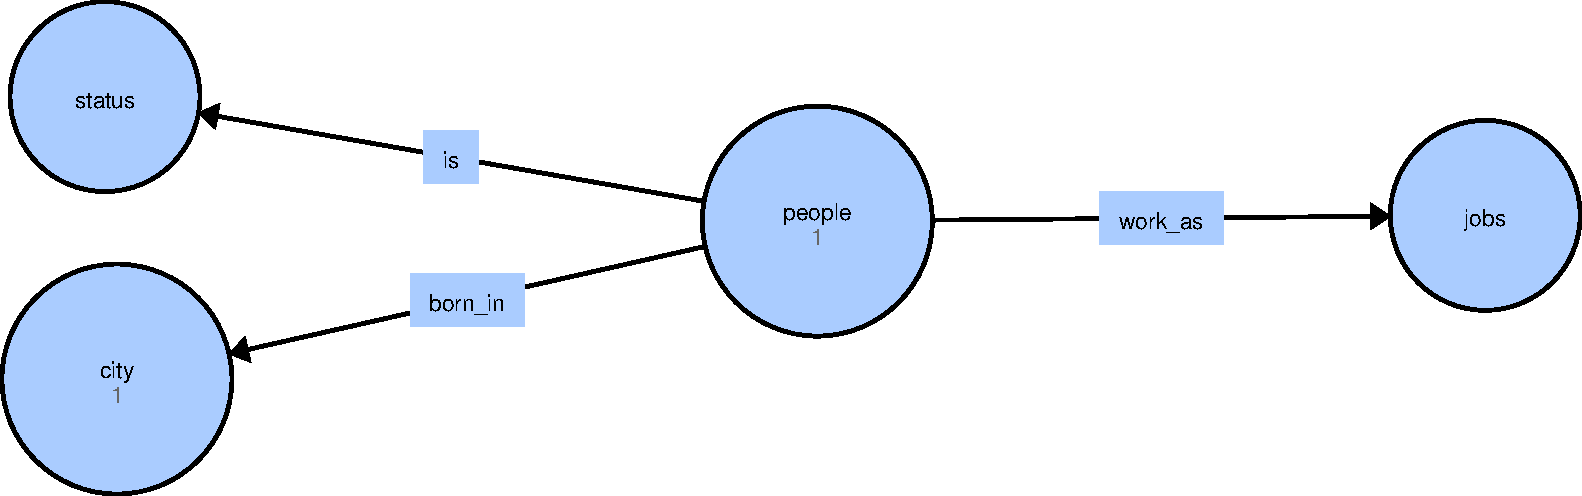
\includegraphics[width=0.6\textwidth]{Picture/society.rdf.pdf}
	\caption{grafo ontologia \texttt{society}}
\end{figure}
\begin{itemize}
	\item \verb|people|: rappresenta gli individui con le loro parentele: rispetto all'ontologia presentata nel listato \ref{lst:persone.rdf} abbiamo aggiunto la relazione simmetrica \verb|marry|, e la relazione \verb|son_of| come inversa di \verb|parent_of|, aggiungiamo anche l'anno di nascita e morte.
\end{itemize}
\begin{figure}[H]
	\centering
	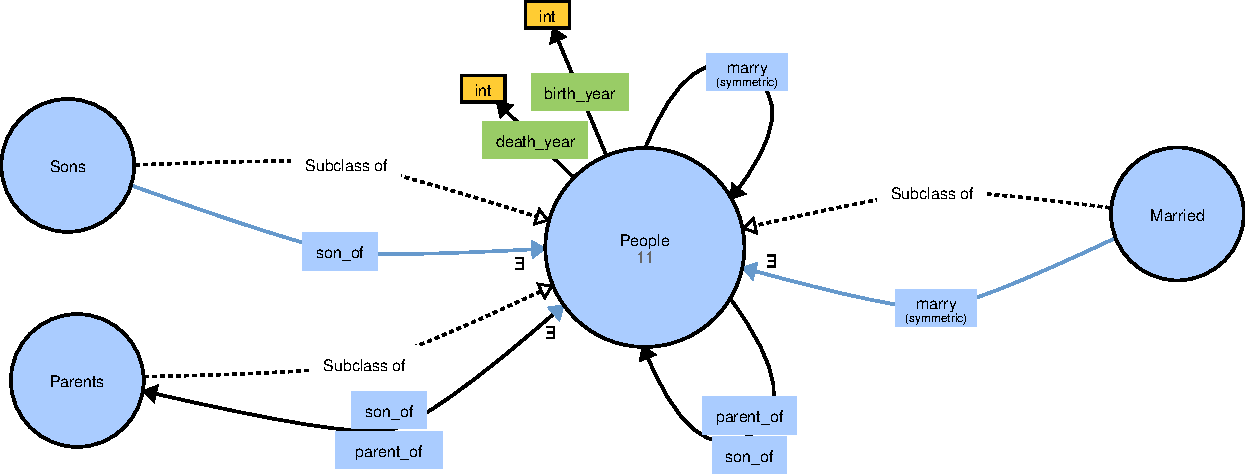
\includegraphics[width=0.75\textwidth]{Picture/people.2.pdf}
	\caption{grafo ontologia \texttt{people}}
\end{figure}
\phantomsection\label{ont_fashion}
\begin{itemize}
	\item \verb|fashion|: è l'ontologia che abbiamo creato nel capitolo \ref{ch3} arricchita con le relazioni \verb|made_of|, \verb|crafted_with|, \verb|color|, che indicano rispettivamente i materiali costituenti, le tecniche realizzative e i colori di un capo d'abbigliamento. Per rappresentare l'ontologia in modo che abbia un'utilità si è deciso di operare un taglio in profondità e ampiezza del grafo, rappresentiamo per ogni classe principale solo il primo livello di sottoclassi, e nel caso questo livello fosse troppo numeroso viene tagliato in ampiezza.
\end{itemize}
\begin{figure}[H]
	\centering	
	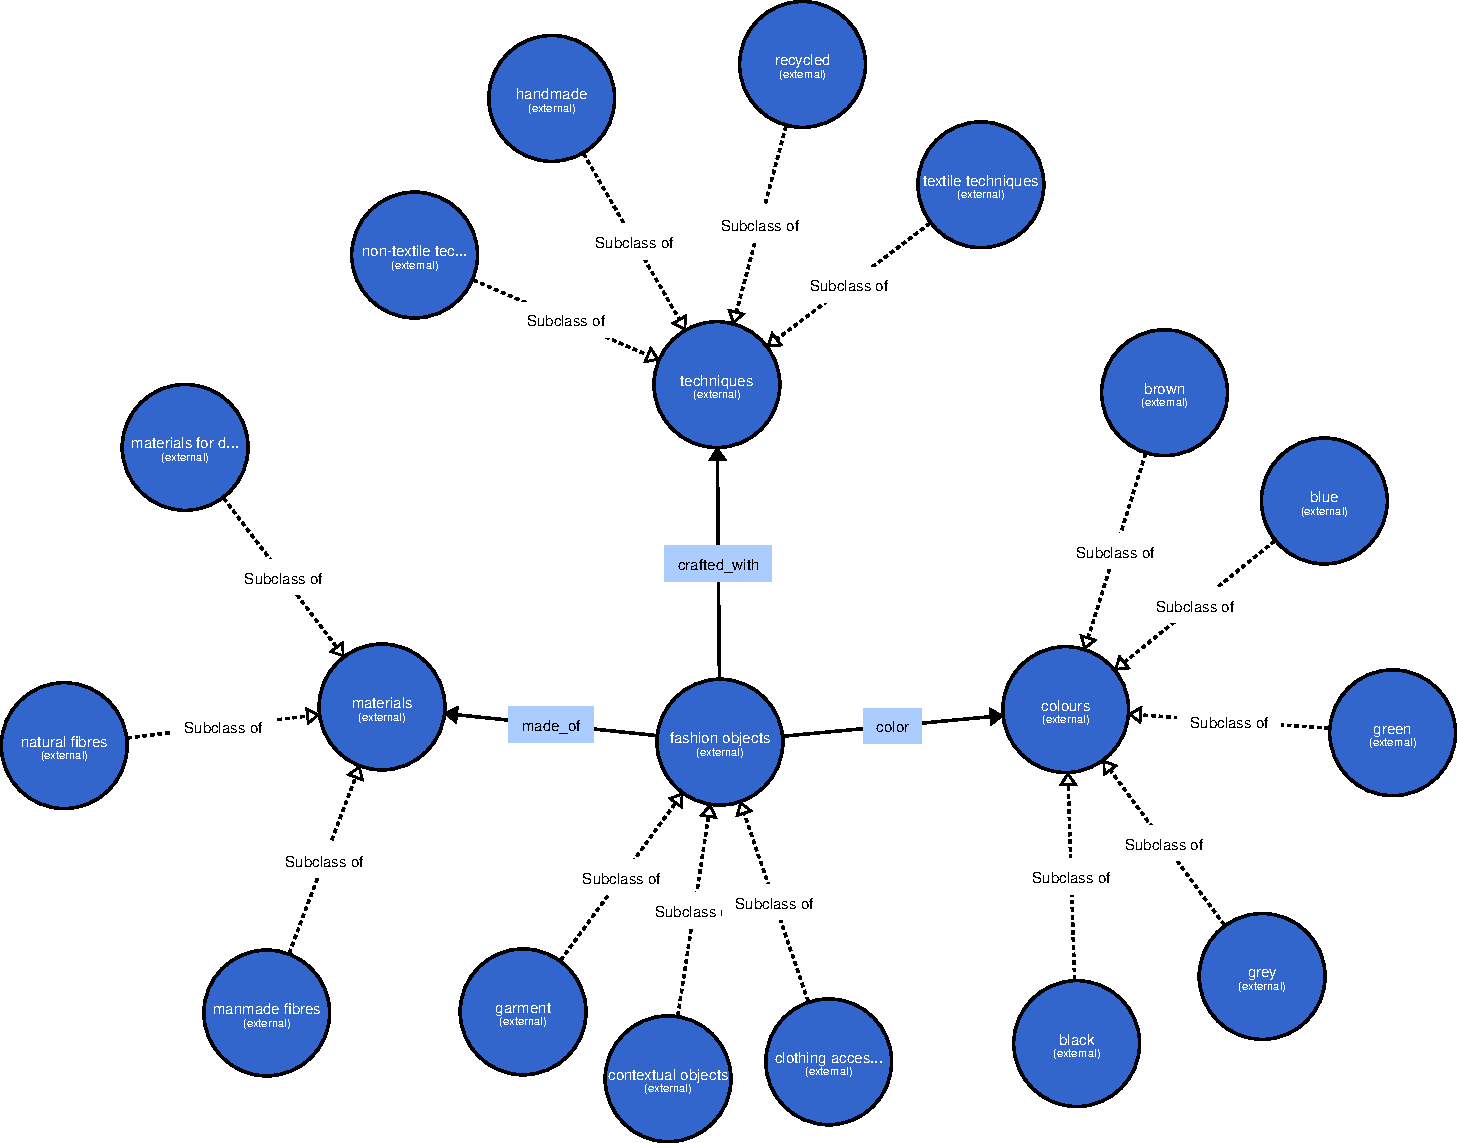
\includegraphics[width=0.65\textwidth]{Picture/europeana_relation.pdf}
	\caption{\label{fig:ontEur}grafo ontologia \texttt{europeana}}
\end{figure}
\subsection{Ontologia di arrivo}
Vogliamo modificare \verb|society| in modo da descrivere gli usi e i costumi della società del XII secolo, per fare questo estrapoliamo dall'ontologia \verb|fashion| tutti i vestiti che non siano costituiti da fibre naturali e scremiamo dall'ontologia \verb|people| tutte le persone che sono vissute in un'epoca che non ci interessa. Vogliamo poi che la classe \verb|People| definita in \verb|society| sia equivalente alla classe \verb|People| definita in \verb|people|, senza perdere tutte le relazioni di parentela, e potendo contemporaneamente sfruttare le nuove relazioni definite in \verb|society|.
\section{Struttura generale di un'ontologia}
Per fare il merge dobbiamo poter caricare le tre ontologie in \cduce, quindi descriviamo una struttura generale per fare il parsing di un'ontologia generica:
\addocaml{general structure}{lst:general_structure}{Code/general_structure.cd}
Rispetto alle strutture definite in precedenza notiamo varie aggiunte:
\begin{itemize}
	\item si specifica meglio l'elemento \verb|EqClass|: questo infatti può essere una restrizione (un genitore è una persona con dei figli) oppure un'equivalenza senza condizioni (ci serve per rendere uguali i concetti di persona definiti nelle due ontologie);
	\item definiamo il tipo \verb|DataProperty|: questo rappresenta una proprietà degli individui, nel nostro caso la usiamo per specificare l'anno di nascita di una persona. Gli individui nella loro lista di attributi potranno ora averne uno di tipo \verb|DataProp|;
	\item il tipo \verb|AnnProperty| serve perché avendo editato l'ontologia \verb|fashion| in Protégé (per aggiungere le relazioni non presenti nel tesauro) i tag SKOS sono stati correttamente riconosciuti \cite{OWL&SKOS} e classificati come tag \verb|owl:AnnotationProperty|;
\end{itemize}
\section{Merge}
\subsection{Funzioni utili}
Prima di passare alla costruzione della nuova ontologia vediamo alcune funzioni utili che si possono applicare a qualsiasi ontologia e che sono servite per costruire le funzioni specifiche adatte a manipolare le particolari ontologie di interesse.
\addocaml{usefull function}{lst:utility.cd}{Code/utility.cd}
Per la prima volta abbiamo fatto ricorso ad applicazioni parziali, questo è utile per poter parametrizzare anche l'ontologia di riferimento; dato che in questo caso ne manipoliamo contemporaneamente tre, è importante poter specificare volta per volta a quale ci riferiamo.

Vediamo per la prima volta degli esempi di funzioni ricorsive:
\begin{itemize}
	\item \verb|andList| e \verb|orList| (linee 22 e 26) lavorano su liste di booleani e restituiscono il risultato della congiunzione o disgiunzione logica tra tutti gli elementi di una lista. Per ottenere questo risultato si fa il pattern matching della lista che può essere un elemento in testa alla lista seguito da una lista che chiamiamo coda; la funzione restituisce l'operazione logica tra la testa e la chiamata ricorsiva alla funzione, passando come parametro la coda della lista. Quando la lista è vuota (seconda clausola del matching) la funzione restituisce l'elemento neutro dell'operazione logica;
	\item \verb|subClassRec| richiama ricorsivamente se stessa per costruire l'intero albero di sottoclassi a partire da una classe data (e dall'ontologia di riferimento). Ovviamente perché questa funzione possa terminare, la struttura delle classi deve essere un grafo aciclico (questa non è una grossa limitazione, infatti se la classe \verb|c2| è contemporaneamente sopraclasse e sottoclasse di \verb|c1|, allora \verb|c1| e \verb|c2| sono equivalenti e possono essere accorpate per eliminare i cicli, discorso analogo vale per cicli più lunghi).
\end{itemize}

Per verificare se un individuo si trova in un certo albero di classi, si potrebbe operare al contrario rispetto a \verb|subClassRec|, risalendo l'albero fino a quando non si trova il padre desiderato (restituendo \verb|true|) oppure la radice delle classi (restituendo \verb|false|). Questo approccio, però, presenta alcune problematiche:
\begin{itemize}
	\item un individuo può appartenere a più classi, quindi bisognerebbe risalire \emph{n} alberi dove \emph{n} è il numero di classi a cui appartiene l'oggetto;
	\item ogni classe può essere sottoclasse di più classi diramando così ulteriormente la ricerca.
\end{itemize}
Facendo alcuni test, si nota che un approccio di questo genere, oltre a essere impegnativo dal punto di vista implementativo, è poco efficiente dal punto di vista prestazionale. Come vedremo nel listato \ref{lst:is_artificial.cd}, per ogni capo d'abbigliamento dovremo chiederci se è costituito da materiali artificiali e questo rallenta il processo di merge. Per evitare questo problema costruiamo solo una volta la lista di materiali artificiali e, quando dobbiamo stabilire se un materiale è naturale o meno, verifichiamo se appartiene alla lista dei materiali artificiali. Questo approccio è vantaggioso in quanto la lista di materiali artificiali andrebbe creata in ogni caso per andare ad aggiungere alla nuova ontologia tutti i materiali che non lo sono (conviene creare la lista dei materiali artificiali piuttosto che quella dei materiali naturali perché la prima contiene molti meno elementi, di conseguenza è più veloce da creare).

Per implementare questa ricerca usiamo \verb|isInClasses| (linea 46) che prende un individuo e una lista di classi, valuta a che classi appartiene l'individuo (con \verb|classOf|) e usa la funzione \verb|contains| per creare una lista di valori booleani uno per ogni classe dell'individuo, verificando se è contenuto nella lista di classi fornita; infine si verifica se la lista di booleani contiene solo \verb|true| con la funzione \verb|andList|.

\subsection{Selezione degli abiti}
Mostriamo come si possano importare solo le fibre naturali e i vestiti costituiti esclusivamente da questi materiali, questo ha lo scopo di presentare come si possa fare della semplice inferenza sulla base di conoscenza usando solamente \cduce e senza ricorrere a reasoner esterni più sofisticati e complessi. Non mostriamo le funzioni per selezionare solo le persone vissute nel periodo storico considerato, questo per non inserire troppo codice e perché sarebbe poco istruttivo (non introdurremmo nuovi concetti rispetto a quelli che presenteremo nel seguito).

Per ragionare sul singolo abito ci domandiamo di che materiali è fatto usando la relazione \verb|made_of| che associa uno o più materiali a un abito. Una volta che abbiamo i materiali, possiamo considerare la struttura ad albero dei materiali dell'ontologia \verb|fashion| (la struttura è quella importata dal tesauro \say{European Fashion Thesaurus}) per distinguere materiali naturali da artificiali (le due categorie devono essere disgiunte). Un vestito verrà considerato valido per la nuova ontologia solo se costituito unicamente da fibre naturali\footnote{Possiamo fare inferenza solo con i dati in nostro possesso, in particolare la classe dei materiali si divide in tre sottoclassi che rappresentano materiali naturali, artificiali e materiali di decorazione; su questi ultimi non possiamo fare alcun ragionamento sull'origine, si è operata una scelta permissiva considerandoli tutti naturali}.

Una possibile implementazione delle funzioni che ci permettono di stabilire se un abito è costituito esclusivamente da fibre naturali è la seguente:
\addocaml{test artificial}{lst:is_artificial.cd}{Code/is_artificial.cd}
La funzione \verb|madeOf| restituisce una lista di individui che sono tutti i materiali di cui è costituito un abito, per fare questo \verb|madeOf| prende come parametri l'abito e l'ontologia di riferimento. 

La funzione \verb|isArtificial| ha due comportamenti differenti a seconda dell'individuo che le viene passato come parametro:
\begin{itemize}
	\item materiale: se l'individuo appartiene all'albero dei materiali, il controllo consiste nello stabilire se questo materiale appartiene alla lista dei materiali artificiali: se è così si restituisce \verb|true|;
	\item indumento: se l'individuo appartiene a una sottoclasse dei vestiti, prima si crea la lista di materiali di cui è costituito, poi si valuta: se almeno uno di questi è artificiale si restituisce \verb|true|.
\end{itemize}
Per poter fare queste operazioni la funzione riceve come parametri: l'individuo da analizzare, la lista di tutti i materiali, la lista dei materiali artificiali e  l'ontologia di riferimento.
\subsection{Costruzione dell'ontologia}
Assembliamo tutti i pezzi visti finora per manipolare l'ontologia \verb|society| aggiungendo tutte le classi e gli individui che ci interessano. Presentiamo subito l'implementazione descrivendola poi passo passo:
\addocaml{assemble ontology}{lst:make_ontology.cd}{Code/make_ontology.cd}
Da linea 1 a linea 3 carichiamo le ontologie che useremo, poi andiamo a creare le liste di classi di materiali che ci servono per utilizzare le funzioni definite nei listati \ref{lst:utility.cd} e \ref{lst:is_artificial.cd}: tutti i materiali e materiali artificiali. Creiamo anche la lista di tutte le classi di vestiti.

Alla riga 9 costruiamo la lista di classi dei materiali ammissibili per la nuova ontologia selezionando dalla lista totale tutti quelli non artificiali. In riga 12 estraiamo tutti i vestiti (individui) costituiti solo da materiali naturali (nella nuova ontologia inseriamo tutte le classi di vestiti, queste possono potenzialmente rappresentare individui fatti di fibre naturali).

Alla linea 17 prendiamo tutti gli elementi dell'ontologia \verb|society| escluso l'elemento di tipo \verb|Ont| e la classe \verb|people|, questo perché l'elemento \verb|Ont| verrà ricreato da zero alla linea 24 e la classe \verb|people| andrà modificata per renderla equivalente alla classe \verb|people| dell'ontologia \verb|people| (linea 20)

In questo esempio prendiamo tutti gli elementi dell'ontologia \verb|people|; come detto prima, presentare il codice per selezionare solo alcune persone sarebbe poco istruttivo. Una volta create tutte le nuove liste di elementi, le assembliamo alla linea 26 e, alla linea 28 costruiamo la nuova ontologia; in riga 30 la salviamo su file.
\subsection{Risultato finale}
L'ontologia che abbiamo costruito permette di descrivere la società nelle modalità che ci eravamo prefissati all'inizio del capitolo (paragrafo \ref{ch4.1}), inoltre abbiamo importato già tutte le persone che avevamo modellato nell'ontologia \verb|people| mantenendo le loro relazioni di parentela; possiamo definire nuove relazioni di parentela sulle persone già modellate in \verb|society| (oppure attribuire loro una data di nascita) e usare le relazioni definite in \verb|society| per arricchire la descrizione di un individuo presente in \verb|people|. Abbiamo anche importato tutte le classi di vestiti e tutti i materiali naturali dall'ontologia \verb|fashion|, possiamo ora creare nuove relazioni tra persone e vestiario  per aggiungere informazioni sugli usi e costumi della società che intendiamo descrivere.

Del risultato finale riportiamo solo la parte di grafo che descrive le persone, la parte che descrive il vestiario è esattamente uguale a quella riportata nell'immagine \ref{fig_eur} alla quale togliamo le fibre artificiali. Il grafo che descrive le persone ci fa apprezzare come effettivamente le due classi estratte, una dall'ontologia \verb|society| e l'altra dall'ontologia \verb|people|, siano effettivamente state accorpate\footnote{In realtà rimangono due classi ma sono dichiarate equivalenti} in un'unica classe che possiede tutti gli attributi e le relazioni delle due classi di partenza.
\begin{figure}[H]
	\centering
	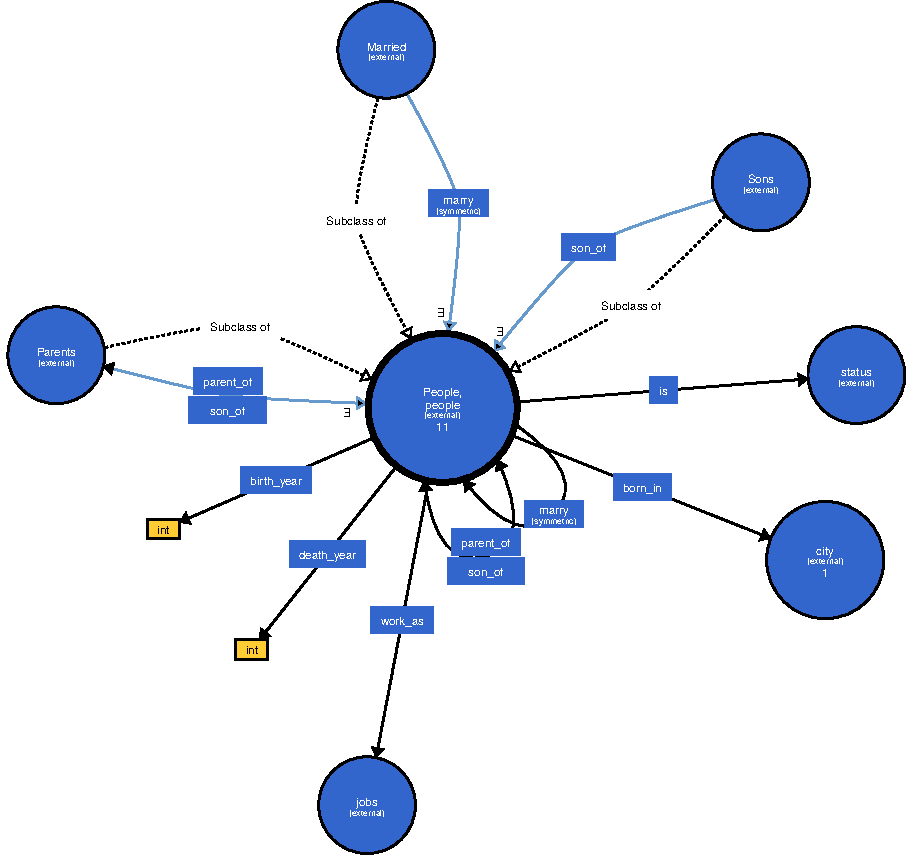
\includegraphics[width=0.8\textwidth]{Picture/society_merged.rdf.pdf}
	\caption{grafo ontologia \texttt{society merged}}
\end{figure}

\section{In Protégé}
In Protégé esiste un comando per fare il merge di ontologie: una volta aperte tutte le ontologie che siamo interessati a fondere, possiamo farne il merge e Protégé si occupa di creare una nuova ontologia e inserire tutte le classi, gli individui, le relazioni e le proprietà di tutte le ontologie di partenza. 

Questo approccio è molto comodo se siamo interessati a prendere tutti i concetti dalle ontologie di partenza, in questo caso l'unico lavoro che ci rimane da fare è quello di mettere in relazione corretta le classi (in questo caso rendere equivalenti le due classi che descrivono le persone). 

Nel caso in cui volessimo fare una selezione più fine su quali concetti importare dovremmo modificare le ontologie di partenza costruendo e scegliendo a prescindere (mediante delle Query) le classi e gli individui che vogliamo importare oppure, una volta fatto il merge, rimuovendo ciò che non ci interessa.
\section{Conclusioni}
Il merge con \cduce richiede di scrivere funzioni che permettano di selezionare cosa importare, questa precisione nella selezione comporta, però, più responsabilità da parte del programmatore che deve fare in modo che i dati continuino a essere consistenti e che le informazioni non vengano alterate durante il merge. Nuovamente sfruttiamo il controllo statico dei tipi offerto da \cduce: in questo caso possiamo notare che man mano che creiamo la nuova ontologia nel listato \ref{lst:make_ontology.cd} verifichiamo che ogni elemento abbia effettivamente il tipo che ci aspettiamo. Controllando il tipo in fase di costruzione siamo sicuri che il documento che salviamo alla fine sia effettivamente un'ontologia e aprendola con un altro strumento (Protégé ad esempio) verrà riconosciuta correttamente e non ci saranno inconsistenze.

Nel caso specifico, il controllo di tipo è stato importante, infatti, la modifica della classe \verb|socPeople| (riga 20 listato \ref{lst:make_ontology.cd}) non era andata a buon fine e aveva generato un elemento XML che non faceva più il match con l'elemento di tipo \verb|Class| (listato \ref{lst:general_structure}). Avremmo comunque potuto salvare il risultato, ma se avessimo tentato di trattarlo come un file che descrive un'ontologia aprendolo con un altro software, avremmo ottenuto un messaggio d'errore (come se il file fosse corrotto) perché il programma non sarebbe stato in grado di interpretare il file come un file \verb|.rdf| ben formato che descrive un'ontologia.


Il merge con Protégé, per quanto lineare, richiede comunque di formulare delle Query più o meno raffinate oppure di eliminare tutto ciò che non serve agli obbiettivi del merge, il processo quindi non è molto più guidato o automatico rispetto alla controparte in \cduce. Come si può vedere dal codice nei listati \ref{lst:utility.cd} e \ref{lst:is_artificial.cd} la maggior parte del lavoro consiste nel creare funzioni che permettano di selezionare cosa importare, una volta fatto questo il codice del listato \ref{lst:make_ontology.cd} che assembla l'ontologia risulta quasi banale. Selezionare elementi con funzioni in \cduce oppure con query in protégé richiede, in entrambi i casi, un certo impegno a livello di programmazione; considerando inoltre che in Protégé una volta selezionati gli elementi con delle Query è comunque necessario eliminare tutti gli altri, \cduce si rivela più efficace potendo importare esattamente ciò che si vuole (a patto di poterlo selezionare).

In conclusione Protégé è uno strumento vantaggioso nei casi in cui si voglia fare il merge tra ontologie mantenendo tutti i concetti rappresentati dalle ontologie di partenza, inoltre manipolando le informazioni con delle Query in Protégé siamo sicuri di ottenere delle ontologie consistenti. Quando è importante selezionare finemente i dati da importare, \cduce si rivela lo strumento migliore, avendo capacità espressiva e manipolativa superiore al set di strumenti base di Protégé (anche in questo caso non prendiamo in considerazione i plug-in che permettono di sviluppare programmi java per manipolare l'ontologia in Protégé). Con il controllo di tipi, \cduce fornisce comunque un certo supporto per verificare che le manipolazioni sulle ontologie portino a strutture consistenti.
	\chapter{Conclusioni}
\section{Maturità di \cduce}
Prima di utilizzare un software in applicazioni importanti è bene domandarsi se lo stesso sia affidabile e vanga manutenuto; questo al fine di evitare situazioni in cui tutto l'applicativo costruito al di sopra di uno strumento crolli al crollare delle fondamenta. Vediamo quindi qual è lo stato di sviluppo di \cduce e quali sono stati le difficoltà tecniche dell'utilizzarlo.
\subsection{Il progetto \cduce}
Come si può leggere nella pagina GitLab del progetto\footnote{https://gitlab.math.univ-paris-diderot.fr/cduce/cduce} \cduce nasce e si sviluppa come una ricerca condivisa tra il gruppo di ricerca sui linguaggi all'ENS\footnote{https://www.ens.psl.eu/} di Parigi e il gruppo di ricerca sui Database all'LRI\footnote{https://www.lri.fr/} ad Orsay. Attualmente il progetto è mantenuto dai PPS laboratory\footnote{https://www.irif.fr/} e dal  Toccata Group\footnote{https://toccata.gitlabpages.inria.fr/toccata/}.

Lo scopo del progetto è quello di costruire un linguaggio per manipolare documenti XML che usi seriamente i tipi XML; questo porta i vantaggi descritti in \ref{fature_cduce}. L'implementazione attuale ha lo scopo di mostrare proprio queste feature innovative e di validare le scelte di progettazione effettuate.
\subsection{Stato di sviluppo attuale}
Sulla pagina del progetto\footnote{https://www.cduce.org/} le ultime informazioni risalgono al 2021 e spiegano che gli sviluppatori si stanno impegnando in una riscrittura completa del compilatore per separare la libreria che gestisce i tipi dal resto del compilatore. La riscrittura del compilatore potrebbe provocare inconsistenza con le ultime versioni di OCaml pertanto si descrive un modo per aggirare il problema oppure si consiglia di utilizzare la vecchia versione. Nonostante le ulime informazioni sul sito siano del 2021 controllando la pagina GitLab si vede che, anche se il branch \say{stable} non riceve aggiornamenti da un anno, altri branch sono tutt'ora attivi\footnote{Alla data in cui si scrive (10/10/2023) l'ultima attività risulta del 09/10/203}.
\subsection{Difficoltà incontrate}
Ho testato \cduce su una distribuzione Ubuntu\footnote{https://ubuntu.com/desktop} e su Arch\footnote{I use Arch btw: https://archlinux.org/}; su Ubuntu non ho avuto successo (seguono dettagli), quindi tutte le prove descritte sono state fatte su Arch.
\subsubsection{Ottenere \cduce}
Sulla pagina del progetto si legge che \cduce è pacchettizzato per le più importanti distribuzioni Linux, ma questi pacchetti, almeno per Ubuntu risalgono a versioni molto vecchie (Ubuntu 12.10 e 13.04) e non funzionano nelle distribuzioni attuali.

Seguendo le istruzioni per compilare la nuova versione (sia polimorfa che monomorfa) di \cduce il processo fallisce, probabilmente questo è dovuto al fatto che da quando è stata scritta la guida ad oggi, i pacchetti di OCaml sono stati ulteriormente aggiornati e il workaround descritto non è più sufficiente. Ho provato, questa volta con successo, ad installare la vecchia versione di \cduce (version 0.6.1-rc1), ho scelto la versione monomorfa perché la versione polimorfa veniva descritta come \say{buggy and experimental}

Il processo di installazione descritto sul sito consiste a grandi linee nel:
\begin{itemize}
	\item creare un ambiente virtuale per OCaml;
	\item installare in questo ambiente le vecchie versioni dei pacchetti necessari a compilare \cduce;
	\item compilare i sorgenti;
	\item ottenere l'eseguibile di \cduce.
\end{itemize}
\subsubsection{Reperire informazioni}
Sul sito si possono trovare molte risorse utilissime per imparare ad usare \cduce, sono presenti in particolare 2 documenti:
\begin{itemize}
	\item una guida utente\footnote{https://www.cduce.org/manual.html} che spiega in modo molto rigoroso l'approccio del linguaggio ai vari tipi, operazioni e funzioni. La spiegazione è molto tecnica, presenta ogni argomento nel modo più generale possibile facendo estensivo uso dei pattern, per leggerla è necessaria qualche base sui linguaggi funzionali e su come il pattern matching operi (soprattutto se si intendono consultare solo alcune sezioni);
	\item un tutorial\footnote{https://www.cduce.org/tutorial.html} che parte direttamente da degli esempi per spiegare il modo in cui \cduce opera. Gli esempi presentati sono molto ben curati e commentati, e permettono di cominciare subito a sperimentare con lo strumento.
\end{itemize}
Entrambe le guide hanno una controparte in PDF molto comoda per poter cercare all'interno dell'intero manuale un certo termine.

Le difficoltà sorgono nel momento in cui siamo interessati a certe sezioni del tutorial, alcune parti mancano per intero, ed essendo uno strumento relativamente di nicchia non c'è un forum o una community estesa alla quale si possa ricorrere per domande o dubbi. Questo rende particolarmente difficile capire certe parti della guida utente che senza esempi risultano particolarmente oscure. In particolare durante gli esperimenti eseguiti è stato importante fare pattern sulle sequenze, questa sezione (come le precedenti di quel capitolo) è assente nel tutorial. Avendo delle basi di Haskell\footnote{https://www.haskell.org/} e cercando di interpretare la guida che è piuttosto criptica in quel capitolo si può provare a immaginare quale sia la struttura corretta per fare il match (è servito nelle funzioni \verb|andList| e \verb|orList| in \ref{lst:utility.cd}).
\subsubsection{Output}
Nei linguaggi funzionali le operazioni di input e output sono sempre delicate, in \cduce per poter esportare un documento XML dobbiamo fare 2 passi: prima trasformiamo l'elemento di tipo \verb|AnyXml| (che contiene il file XML che vogliamo salvate) in una stringa poi facciamo il dump della stringa su file. Per la conversione da XML a stringa abbiamo 2 possibilità, se il documento contiene solo caratteri previsti dalla norma  ISO-8859-1\footnote{https://www.iso.org/standard/28245.html} si può usare \verb|print_xml| altrimenti per preservare tutti i caratteri si usa \verb|print_xml_utf8|. Ottenuta la stringa si può fare il dump su file con \verb|dump_to_file| oppure \verb|dump_to_file_utf8|, questo sarà un file XML che nel nostro caso rappresenta un ontologia.

Provando ad aprire il risultato di un dump con un editor di testo ci si tende conto che tutto il codice XML si trova su una sola riga, manca completamente qualsiasi formattazione e il file risulta dunque illeggibile. Aprendo il file con uno strumento come Protégé non ci sono problemi, il file è ben formato e viene interpetato correttamente, ma se vogliamo vedere il risultato della manipolazione con \cduce senza ricorrere ad altri software appositi ci troviamo in difficoltà\footnote{Senza contare che Protégé quando si salva il file sul quale si ha lavorato sì lo riformatta correttamente, ma riposiziona gli elementi e aggiunge parti non presenti in origine (anche semplicemente i commenti) rendendo imossibile conoscere il documento originale}. Se siamo intenzionati a vedere il risultato del dump di \cduce dobbiamo riformattare il documento per renderlo fruibile. Per fare questo ci sono molte opzioni, in questo caso è stato sviluppato un piccolo programma in java che riformatta il file XML rendendo possibile un'ispezione dello stesso mediante un editor di testo. 

Il problema è probabilmente dovuto al fatto che le funzioni di \verb|pretty-printing| di \cduce usano per le funzioni di OCaml, avendo forzato l'allineamento tra i pacchetti di OCaml e \cduce è possibile che non sia tutto esattamente compatibile, questo fa sì che le componenti non funzionali di \cduce e in generale l'interazione tra \cduce e OCaml non funzioni correttamente.

È in ogni caso un peccato che attualmente l'unico modo per poter leggere il risultato dell'esecuzione di un programma scritto con un linguaggio funzionale, usato senza ricorrere a nessuno stratagemma imperativo, richieda l'esecuzione di un programma in java per rendere leggibile il risultato.
\subsection{Sviluppi futuri}
Considerando che il progetto sembra essere ancora di interesse per i gruppi di ricerca che vi hanno lavorato e che il repository risulta attivo ed utilizzato è auspicabile che la riscrittura del compilatore iniziata nel 2021 termini e la nuova versione di \cduce sia polimorfa e sfrutti l'ultima versione di OCaml, questo ridurrebbe drasticamente i problemi descritti sopra e potrebbe spingere più persone ad interessarsi al progetto e a collaborare per rendere \cduce uno strumento professionale a tutti gli effetti; attualmente \cduce viene considerato dagli sviluppatori stessi come un prototipo di ricerca e non adatto ad applicazioni stabili\footnote{https://gitlab.math.univ-paris-diderot.fr/cduce/cduce/-/wikis/home}.
\section{Punti di forza di \cduce}
Nonostante le difficoltà incontrate \cduce si è rivelato uno strumento molto potente e versatile per la manipolazione di ontologie, in particolare il fatto di essere un linguaggio funzionale lo rende particolarmente sintetico e leggibile una volta presa dimestichezza coi concetti base.
\subsection{Sistema di tipi}
I tipi descrivono un insieme di valori costruiti in un certo modo, è estremamente facile definire un tipo e la sua struttura, d'altra parte avere dei tipi definiti correttamente ci permette di scrivere funzioni che li manipolano come ci aspettiamo e che restituiscono un elemento esattamente del tipo che vogliamo.

Tutta la verifica dei tipi in \cduce avviene staticamente, saremo quindi sicuri che una funzione trasformi un concetto di un tesauro in una classe di un'ontologia ancora prima di eseguire questa funzione perché \cduce verifica che tutte le trasformazioni che applichiamo permettano di passare da un elemento del primo tipo ad un elemento del secondo.

Il controllo di tipo avviene per tutte le funzioni che definiamo (a patto di specificarne correttamente l'interfaccia) e permette di scrivere del codice in cui la maggior parte del debugging possa essere fatta in fase compilazione e non a run-time. 

\subsection{Funzioni di ordine superiore}
Come tutti i linguaggi funzionali anche \cduce permette di definire funzioni di ordine superiore, queste hanno numerosi vantaggi: 
\begin{itemize}
	\item possiamo scrivere funzioni semplici di cui è facile verificare la correttezza e assemblarle in funzioni più articolate che diventano più trattabili, gestendo in questo modo la complessità;
	\item le funzioni di ordine superiore permettono di generalizzare il codice in modo estremamente efficace, consideriamo il caso di una funzione che rimuove alcuni elementi di una lista secondo un certo criterio, nel momento in cui cambia il criterio dovremmo riscrivere almeno parte della funzione, se invece implementiamo un una funzione per la rimozione selettiva che fra i vari parametri accetta una funzione che specifica se un elemento della lista va eliminato possiamo scrivere una funzione assolutamente generale che possa lavorare con un qualsiasi criterio che andremo volta per volta a specificare. Su questa possibilità torneremo dopo in \ref{ch5.4_func}
\end{itemize}
\subsection{Pattern matching}
Grazie al pattern matching è possibile effettuare complesse operazioni di estrazione dei dati e manipolazione degli stessi, è un aspetto centrale di \cduce e ne incrementa moltissimo la potenza espressiva. Purtroppo non è lo strumento più semplice da padroneggiare e ad una prima vista può sembrare ambiguo il modo in cui descrivere un certo pattern. Lievi differenze nella definizione del pattern producono effetti differenti, e bisogna prestare particolare attenzione a descrizioni che apparentemente possono sembrare equivalenti.
\section{Spunti per paragoni futuri}
In questo lavoro abbiamo provato a fare dei paragoni tra \cduce e Protégé, sono due strumenti molto differenti e le scale di paragone, a seconda dei parametri considerati, fanno risaltare uno strumento come molto efficace e l'altro come inappropriato. Potrebbe essere quindi interessante confrontare \cduce con altri strumenti più simili.
\subsection{Confronto con un linguaggio imperativo}
Esistono vari linguaggi che incorporano librerie per la modellazione di documenti XML, uno fra tutti è sicuramente java.
\subsubsection{JAXP}
JAXP\cite{JAXP} è l'API che java mette a disposizione per processare dati in XML. I packages contenuti in questa API consentodo alle applicazioni di fare il parsing, trasformare, validare e interrogare con delle query documenti XML. JASP è dotata di un layer che permetta l'indipendenza tra il codice dell'applicazione e il particolare processor XML implementato. JAXP, rispetto a \cduce che è attualmente in stato di sviluppo ed è considerato un prototipo, garantisce la possibilità di sviluppare applicazioni per il processing di file XML che siano perfettamente funzionanti, integrabili e stabili.

Alla luce dei vantaggi di affidabilità offerti da progetti molto più grandi di \cduce potrebbe essere interessante valutare come l'uso di un linguaggio funzionale possa apportare benefici a livello di programmazione, correttezza del codice e leggibilità rispetto ad un linguaggio essenzialmente imperativo come java.
\subsection{Confronto con un linguaggio funzionale}
\cduce nasce con lo scopo di processare documenti XML, esistono altri linguaggi più general porpouse che implementano la capacità di elaborare XML tramite librerie. Uno dei linguaggi che presenta ampia scelta di librerie è Haskell. Questo linguaggio è sicuramente più noto di \cduce e sono disponibili, pertanto, numerose risorse online per chiarire domande e dubbi che possono sorgere. Fra le librerie per l'elaborazione di documenti XML citiamo HaXml\footnote{https://archives.haskell.org/projects.haskell.org/HaXml/} e Haskell XML Toolbox (HXT)\footnote{https://wiki.haskell.org/HXT}, che si basa sulle idee di HaXml, entrambi i progetti risultano attivi e documentati.

Il vantaggio di usare una di queste librerie è la possibilità di interfacciarsi direttamente con Haskell potendo integrare le funzionalità della libreria scelta con le numerosissime funzioni offerte da Haskell (sia prese dai pacchetti base sia implementate da librerie esterne). Anche \cduce dovrebbe fornire integrazione con OCaml sia permettendo di richiamare OCaml in \cduce sia viceversa: attualmente, almeno dalle prove effettuate, non risulta, però, possibile integrare i due strumenti.
\subsection{Confronti possibili}
Abbiamo presentato altri strumenti alternativi a \cduce, i confronti possibili potrebbero basarsi sulle seguenti caratteristiche
\begin{itemize}
	\item velocità di sviluppo del codice: ci aspettiamo che un linguaggio funzionale possa presentare dei vantaggi soprattutto nell'esprimere delle trasformazioni degli elementi rispetto ad un linguaggio imperativo; sfruttando poi la funzione \verb|map| (sia in \cduce che Haskell) risulta anche immediato appplicare la trasformazione ad intere liste di elementi;
	\item correttezza del software: anche in questo caso un linguaggio funzionale che esegua un controllo statico dei tipi in fase di compilazione può aiutarci ad evidenziare errori prima che si presentino a run-time;
	\item scalabilità e integrazione: probabilmente da questo punto di vista un linguaggio come java offre dei vantaggi essendo pensato per anche per lo sviluppo di applicativi di grandi dimensioni più che Haskell o \cduce (in ogni caso nulla vieta di integrare \cduce in applicazioni scritte in altri linguaggi, questa possibilità è approfondita in \ref{ch5.4});
	\item  velocità di esecuzione: durante gli esperimenti si è notato un drastico rallentamento dell'esecuzione quando si usavano funzioni ricorsive per creare gli insiemi di sottoclassi, può essere utile provare almeno in java ad implementare una versione iterativa dello stesso algoritmo per verificare se le prestazioni cambiano significativamente. Per quanto riguarda le query può essere interessante un confronto dato che queste ultime in \cduce sono ottimizzate con le stesse tecniche di ottimizzazione della logica classica SQL.
\end{itemize}
\section{Sviluppo di nuovi strumenti}
\subsection{Criticità di \cduce}
\cduce si è rivelato essere un valido e potente strumento per la manipolazione di file XML; a prescindere dai problemi riscontrati durante gli esperimenti, che auspicabilmente verranno tutti risolti con il rilascio della nova versione stabile, la più grande difficoltà che un utente incontra quando si approccia all'uso di questo strumento è proprio la difficoltà di esprimere degli algoritmi con un linguaggio funzionale.

Se chi vuole usare \cduce per manipolare delle ontologie non ha grandi competenze in campo di programmazione ed ha usato fino a quel momento solo strumenti grafici per la creazione o manipolazione di ontologie si scontra con una notevole difficoltà di sviluppo degli strumenti, che solo in parte sono guidate dal tutorial presente sul sito, in numerosi casi bisogna essere in grado di interpretare la guida che ad un utente non esperto può sembrare poco chiara.

Discorso analogo vale per un utente già competente nell'uso di linguaggi imperativi che si trova a dover fare i conti con un nuovo paradigma di programmazione senza che la guida o il tutorial aiutino particolarmente. Probabilmente un utente di questo tipo si troverà ancora più confuso di un utente novizio alla programmazione.

\cduce presuppone che i suoi utenti posseggano delle competenze già abbastanza avanzate nell'uso di linguaggi funzionali, che si trovino a proprio agio nello sviluppare algoritmi ricorsivi e ad usare intensivamente il pattern matching. Date le competenze richieste e la curva d'apprendimento particolarmente ripida \cduce potrebbe rivelarsi uno strumento ostico per la maggior parte degli utenti che vogliono concentrarsi sulla creazione di un'ontologia che sia corretta e ben formata e non sullo sviluppo di codice per la creazione stessa.

\subsection{Interfaccia grafica}\label{ch5.4}
Fatte le precedenti considerazioni ne risulta che nonostante \cduce sia uno strumento potente ed espressivo sia anche particolarmente poco fruibile. Per arginare la difficoltà d'uso si potrebbe pensare ad un interfaccia che permetta di rendere grafiche la maggior parte delle operazioni, relegando la parte di programmazione a task specifici o che operano ad hoc sulla particolare ontologia che si sta manipolando.

Esistono numerose interfacce da cui trarre ispirazione\footnote{Se la creazione di una nuova interfaccia da zero rappresenta un ostacolo eccessivo, si può pensare di costruire in \cduce dei plug-in per Protégé} (l'interfaccia di Protégé per citarne una) e \cduce si presta particolarmente bene a creare codice generale:
\begin{itemize}
	\item parsing di una generica ontologia: come si può notare in \ref{lst:general_structure} la struttura definita permette di fare correttamente il parsing di tre ontologie completamente differenti, la struttura non è esaustiva e si potrebbero dover aggiungere altre definizioni di tipi per renderla completamente generale senza rinunciare ai controlli di correttezza\footnote{Se si usasse il tipo \texttt{AnyXml} la struttura sarebbe generalissima ma non offrirebbe più controlli puntuali sulla correttezza dei tipi ritornati dalle funzioni}; questa aggiunta risulta, in ogni caso, fattibile e non dispendiosa;
	\item funzioni generali per trattare con ontologie: guardando il codice in \ref{lst:utility.cd} ci si rende conto che queste funzioni non hanno alcuna attinenza con le particolari ontologie che stiamo trattando, un parco sufficientemente ampio di queste funzioni sarebbe in grado di estrarre la maggior parte delle informazioni utili da un ontologia, di selezionare e di assemblare le parti che l'utente vorrebbe poter mantenere;
	\phantomsection
	\item\label{ch5.4_func}funzioni di ordine superiore: laddove le funzioni generali non bastano si potrebbero pensare funzioni di ordine superiore complesse a piacere che servano per manipolare in modo molto specifico le ontologie che si stanno trattando, queste funzioni vengono messe a disposizione dell'utente che deve solo integrare piccole e semplici funzioni che prese come argomento dalla funzione di ordine superiore la rendano specifica per la particolare ontologia d'interesse. Questo limita notevolmente la necessità di programmare dell'utente anche quando si voglia costruire degli strumenti molto specifici per la propria ontologia;
	\item creazione guidata di query: esistono già numerosi strumenti che permettono la creazione di query, anche particolarmente complesse, in modo grafico e guidato; data la profonda somiglianza tra le query espresse in linguaggio SQL e la sintassi in \cduce sarebbe possibile riproporre uno strumento del genere per rendere le query accessibili.	
\end{itemize}
\section{Conclusioni}
\cduce nonostante sia classificato come prototipo è uno strumento per la manipolazione di documenti XML ed in particolare di ontologie completo ed espressivo\footnote{Si fa riferimento alla versione del software 0.6.1-rc1}. Offre una documentazione online ben curate e accessibile ad un utente con solide basi di programmazione funzionale, la documentazione è inoltre accompagnata da una serie di esempi che guidano, almeno fino ad un certo punto, un utente più novizio a muovere i primi passi con lo strumento potendo già realizzare programmi utili.

Paragonandolo ad altri strumenti si rivela acerbo e il sito riflette questa condizione essendo finito solo per metà (numerosi link e componenti non sono attualmente funzionanti). Nonostante questo, rispetto a software molto più grandi e più specificatamente orientati alla manipolazione di ontologie \cduce permette di esprimere una grande quantità di lavoro in poche righe di codice, in modo elegante e leggibile. 

L'elaborazione di molti dati, la selezione secondo certi criteri e la trasformazione di elementi seguendo certi pattern risulta molto naturale in questo linguaggio; questi vantaggi e il controllo statico su tipi che garantisce la costruzione di ontologie ben formate rendono \cduce uno strumento efficace nella manipolazione di ontologie, e anche se non è uno strumento specifico per questo scopo, si dimostra, in certi casi d'uso, più potente di Protégé. 
	\newpage
	
	\listoflistings
	
	\printbibliography
	
\end{document}